% use paper, or submit
% use 11 pt (preferred), 12 pt, or 10 pt only

\documentclass[letterpaper, preprint, paper,11pt]{AAS}	% for preprint proceedings
%\documentclass[letterpaper, paper,11pt]{AAS}		% for final proceedings (20-page limit)
%\documentclass[letterpaper, paper,12pt]{AAS}		% for final proceedings (20-page limit)
%\documentclass[letterpaper, paper,10pt]{AAS}		% for final proceedings (20-page limit)
%\documentclass[letterpaper, submit]{AAS}			% to submit to JAS

\usepackage{bm}
\usepackage{amsmath}
\usepackage{amssymb}
\usepackage{physics}
\usepackage{algorithm}
\usepackage{algpseudocodex}
\usepackage{subfigure}
\usepackage{float}
%\usepackage[notref,notcite]{showkeys}  % use this to temporarily show labels
\usepackage[colorlinks=true, pdfstartview=FitV, linkcolor=black, citecolor= black, urlcolor= black]{hyperref}
\usepackage{overcite}
\usepackage{footnpag}			      	% make footnote symbols restart on each page

\DeclareMathOperator*{\argmin}{arg\,min}
\newcommand{\R}{\mathbb{R}}
\newcommand{\E}{\mathbb{E}}
\let\P\relax\newcommand{\P}[1]{\mathbb{P}\left[#1\right]}

\PaperNumber{25-624}

\begin{document}

\title{Cislunar Maneuvering Low-Thrust Spacecraft Tracking with Adaptive Optimal Control Estimation}

\author{Darin D. Lin\thanks{M.S. Student, School of Aeronautics and Astronautics, Purdue University, West Lafayette, IN 47906},  
Kenshiro Oguri\thanks{Assistant Professor, School of Aeronautics and Astronautics, Purdue University, West Lafayette, IN 47906}}


\maketitle{} 		


\begin{abstract}
%The abstract should briefly state the purpose of the manuscript, the problem to be addressed, the approach taken, and the nature of results or conclusions that can be expected. It should stand independently and tell enough about the manuscript to permit the reader to decide whether the subject is of specific interest. The abstract shall be typed single space, justified, centered, and with a column width of 4.5 inches. The abstract is not preceded by a heading of ``Abstract'' and its length may not extend beyond the first page.
Tracking maneuvering cislunar spacecraft is a difficult task due to the highly nonlinear dynamical environment, great distances, and frequent observation gaps. If optimal control is assumed, it is possible to predict the future control of a spacecraft given observations of the start of a maneuver. This idea is applied to construct an optimal control interacting multiple model estimator (OCIMM) by including the costate as an estimation variable. The OCIMM can significantly reduce the mean absolute estimation error compared to a traditional IMM during observation gaps and periods of rapidly changing control through its ability to predict the future control. 
\end{abstract}


\section{Introduction}

%This is going to be pretty similar to most other papers on cislunar SDA. Will need to cite many papers here, including Iannamorelli, Holzinger, Scheeres, Wishnek, and Lubey. Discuss other efforts in cislunar SDA, optimal-control based estimation, cislunar initial orbit determination, and maneuver reconstruction.

International interest in cislunar space has increased significantly in the recent decade \cite{nelson2024moon}. Space domain awareness (SDA) will be critical for the future sustainable development of cislunar space. Compared to SDA near Earth, cislunar SDA faces significant challenges due to highly nonlinear cislunar dynamics, extreme distances, and frequent observation gaps. To add to this complexity, active cislunar spacecraft have the ability to maneuver, which in combintation with the chaotic cislunar dynamics further compounds the extreme nonlinearity of the tracking problem. Additionally, low-thrust propulsion has become an increasingly popular choice for spacecraft because of its high specific impulse, allowing for longer mission durations and smaller fuel fractions. Thus, tracking low-thrust maneuvering spacecraft in cislunar space is a problem of interest. 

Significant research effort has been dedicated to the general maneuvering target tracking problem. Bar-Shalom et al. presents several sequential algorithms to account for the discrete nature of maneuvering objects, most notably the interacting multiple model estimator \cite{bar1989tracking} (IMM) and the variable state dimension estimator \cite{bar2007variable} (VSD). Goff et al. implements a combination of these algorithms specifically for tracking low-thrust maneuvering spacecraft in geocentric orbits \cite{goff2015orbit}. Wetterer et al. utilizes an IMM to track impulsively maneuvering spacecraft in cislunar space \cite{wetterer2022cislunar}.

Other research efforts have been dedicated to manage the nonlinearity of the problem. DeMars et al. model the true uncertainty distribution as a mixture of Gaussian distributions, where the number of Gaussian kernels is adaptively increased and decreased in areas of higher and lower nonlinearity, respectively, where nonlinearity is detected via entropy \cite{demars2013entropy}. They then apply this algorithm to accurately model the uncertainty distribution of a spacecraft in geocentric orbit. Vishwjeet and Singla similarly apply a Gaussian mixture-based approach, instead detecting nonlinearity using the Kolmogorov equation error \cite{vishwajet2018adaptive}. 

\begin{figure}
    \centering
    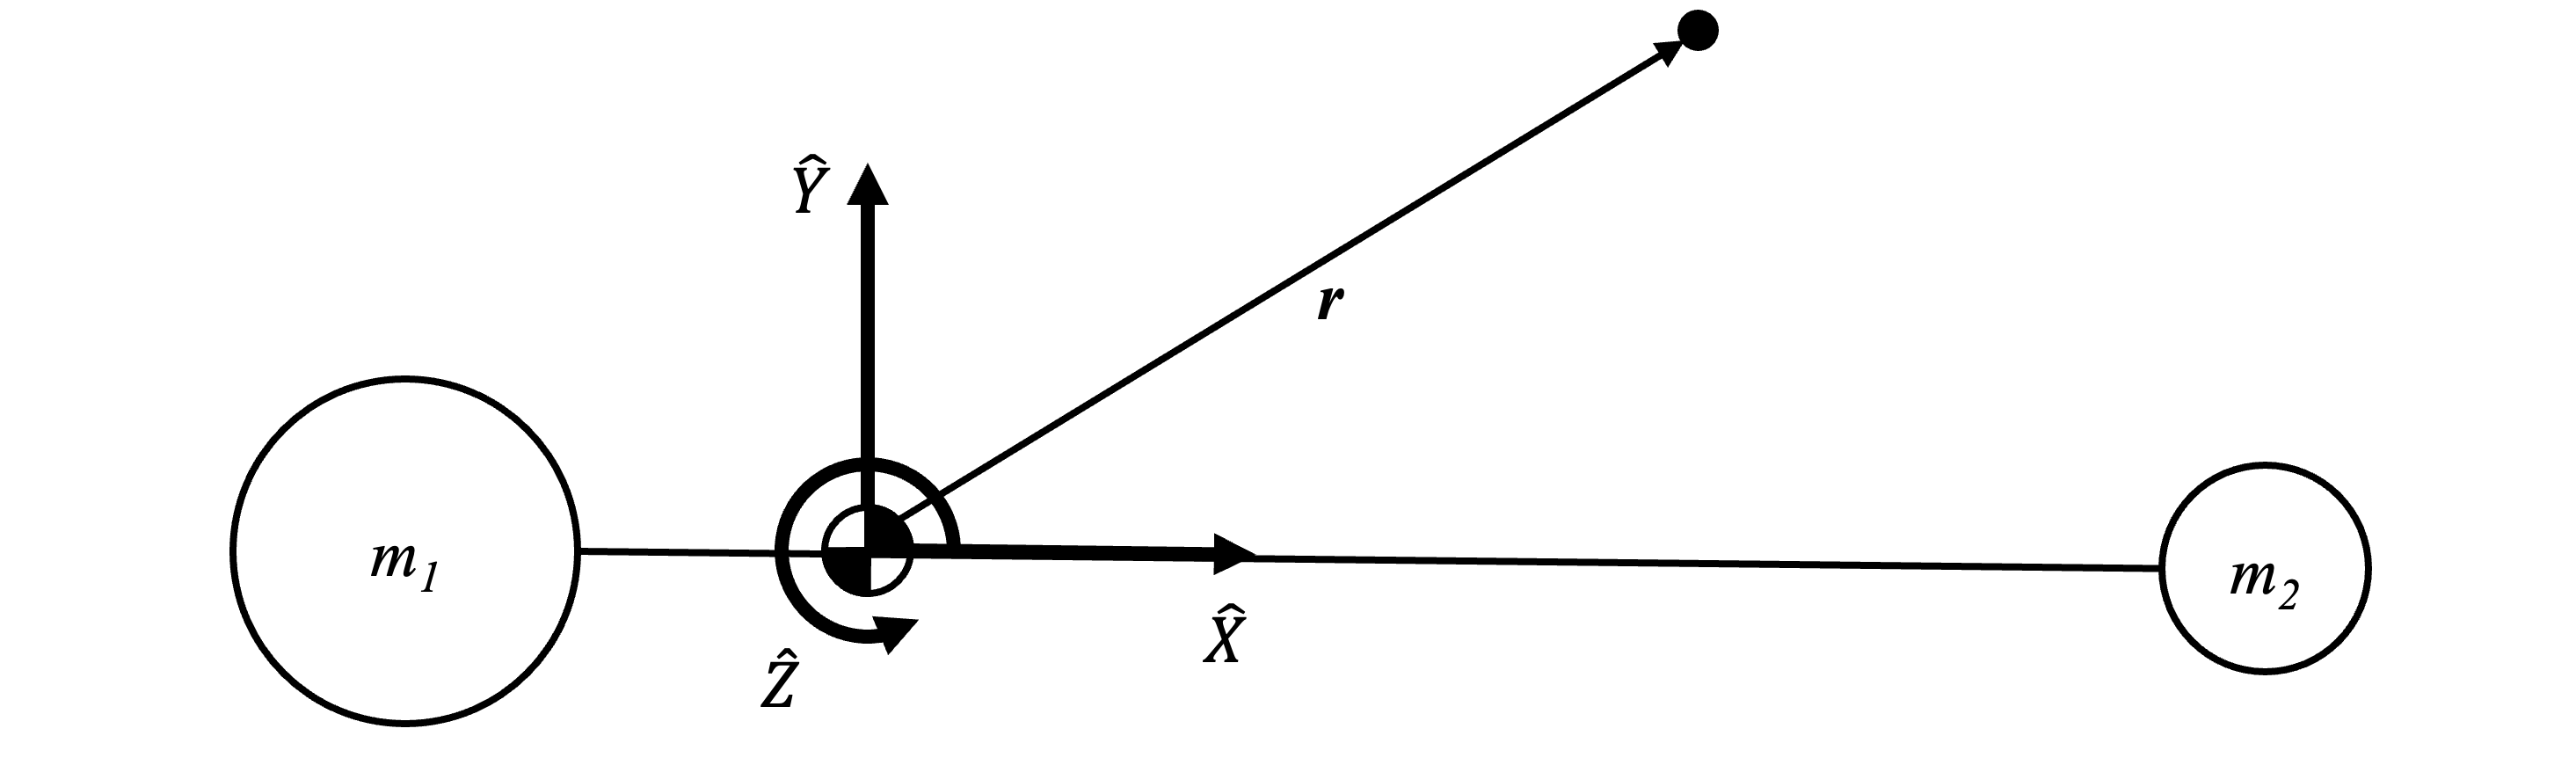
\includegraphics[width=1\linewidth]{Figures/CR3BP.png}
    \caption{Circular-Restricted Three-Body Problem Coordinate Frame}
    \label{fig:CR3BP}
\end{figure}

Iannamorelli and LeGrand combine the adaptive Gaussian mixture and multiple model estimation approaches to simultaneously combat the extreme nonlinearity of cislunar dynamics and account for the maneuvers of a spacecraft \cite{iannamorelli2025adaptive}. Their adaptive Gaussian mixture interacting multiple model estimator (AGMIMM) models maneuvers as zero-mean, Gaussian process noise, so if properly tuned to capture all possible spacecraft maneuvers, the AGMIMM is able to accurately determine where the spacecraft \textit{could} be. However, it is reasonable to assume that the maneuvers of the target spacecraft will be optimal, in which case modeling maneuvers as zero-mean process noise would be overly-conservative. If instead some optimal control law is assumed, given observations of the beginning of a maneuver, it is possible to predict where the spacecraft \textit{should} be at some future time with less uncertainty than by modeling maneuvers as zero-mean process noise. As cislunar SDA becomes more complex with more cislunar spacecraft, decreasing this uncertainty will be critical for correlating tracks of multiple maneuvering targets and allocating limited observational resources.

The concept of using optimal control to improve tracking is explored by Holzinger et al., resulting in the development of the control-distance metric \cite{holzinger2012object}. The control-distance metric characterizes the amount of control effort required to connect two spacecraft states assuming some optimal control, thus allowing the correlation of tracks which are separated by smaller control distances. Lubey and Scheeres apply this framework to develop a sequential estimator, resulting in the Optimal Control-Based Estimator (OCBE) \cite{lubey2013optimal}. The OCBE models any deviation in the state dynamics as an optimal control, which allows both control inputs and mismodeled dynamics to be reconstructed from these deviations. The OCBE is applied by Greaves and Scheeres to the cislunar tracking problem for maneuver detection and reconstruction \cite{greaves2021observation}. These approaches, however, are for the posterior reconstruction and detection of maneuvers rather than for the prior prediction of maneuvers. 

The main contribution of this paper is the implementation of an assumed optimal control policy directly into the dynamics of an adaptive multiple-model estimator. An IMM with two modes is utilized, where the non-maneuvering (coasting) mode assumes ballistic dynamics, and the maneuvering (thrusting) mode assumes a minimum-time optimal control policy. The dynamics of the minimum-time optimal control policy are obtained using Pontryagin's minimum principle \cite{pontryagin1962}. This optimal control IMM (OCIMM) is used to track a cislunar spacecraft performing a low-thrust transfer between two periodic cislunar orbits under a fuel-optimal control policy, whose thrusting arcs follow the same dynamics of a time-optimal policy. The OCIMM is shown to be able to accurately predict the future control inputs of the target spacecraft, even during observation gaps and periods of rapidly changing control. This results in superior estimation performance compared to a traditional IMM. 

\section{Background}

\subsection{Circular-Restricted Three-Body Problem (CR3BP) with Control}

To model the motion of a maneuvering spacecraft in cislunar space, we utilize the circular restricted three-body problem dynamics model with low-thrust control modeled as an affine acceleration. This model assumes circular motion of two massive primary bodies around their barycenter. A third massless body is then subject to the gravities of the other two massive bodies. This third body represents the spacecraft of interest, and its state $\bm{\xi} = [\bm{r}^\top, \bm{v}^\top]^\top$ consists of a three-dimensional position and velocity, $\bm{r} = [x, y, z]^\top$ and $\bm{v} = [v_x, v_y, v_z]^\top$, respectively. The control is a three-dimensional additive acceleration $\bm{u} = [u_x, u_y, u_z]^\top$. To define the coordinate frame, the origin is fixed at the barycenter, the X-axis is aligned with the line between the two massive bodies, the Z-axis is aligned with the angular velocity vector, and the Y-axis completes the X-Y-Z right-handed coordinate frame. The CR3BP coordinate frame is illustrated in Figure \ref{fig:CR3BP}. 

The units of the system are normalized such that the unit length is the distance between the two massive bodies, and the unit time is the inverse of the angular velocity of the two massive bodies. The motion of the massless body is then described by a system of nonlinear differential equations given by 
\begin{align}
\begin{aligned}
    \dot{\bm{\xi}} &= \bm{g}(\bm{\xi}) + B\bm{u}= \begin{bmatrix}
        v_x \\
        v_y \\
        v_z \\
        -\frac{(1 - \mu)(x + \mu)}{d^2} - \frac{\mu(x + \mu - 1)}{r^2} + 2v_y + x\\
        -\frac{(1 - \mu)y}{d^2} - \frac{\mu y}{r^2} - 2v_x + y\\
        -\frac{(1 - \mu)z}{d^2} - \frac{\mu z}{r^2}
    \end{bmatrix} + \begin{bmatrix}
        0_{3 \times 3} \\
        I_3
    \end{bmatrix} \begin{bmatrix}
        u_x \\
        u_y \\
        u_z
    \end{bmatrix} \\
    d &= \sqrt{(x+\mu)^2 + y^2 + z^2}, \quad r = \sqrt{(x + \mu - 1)^2 + y^2 + z^2} \label{eq:CR3BP-dynamics}
\end{aligned}
\end{align}
\noindent where $\mu = m_2/(m_1 + m_2)$ is the ratio of the second body's mass to the total mass of the system \cite{zimovan2017characteristics}.

\subsection{Periodic Orbits in the CR3BP}

\begin{figure}
    \centering
    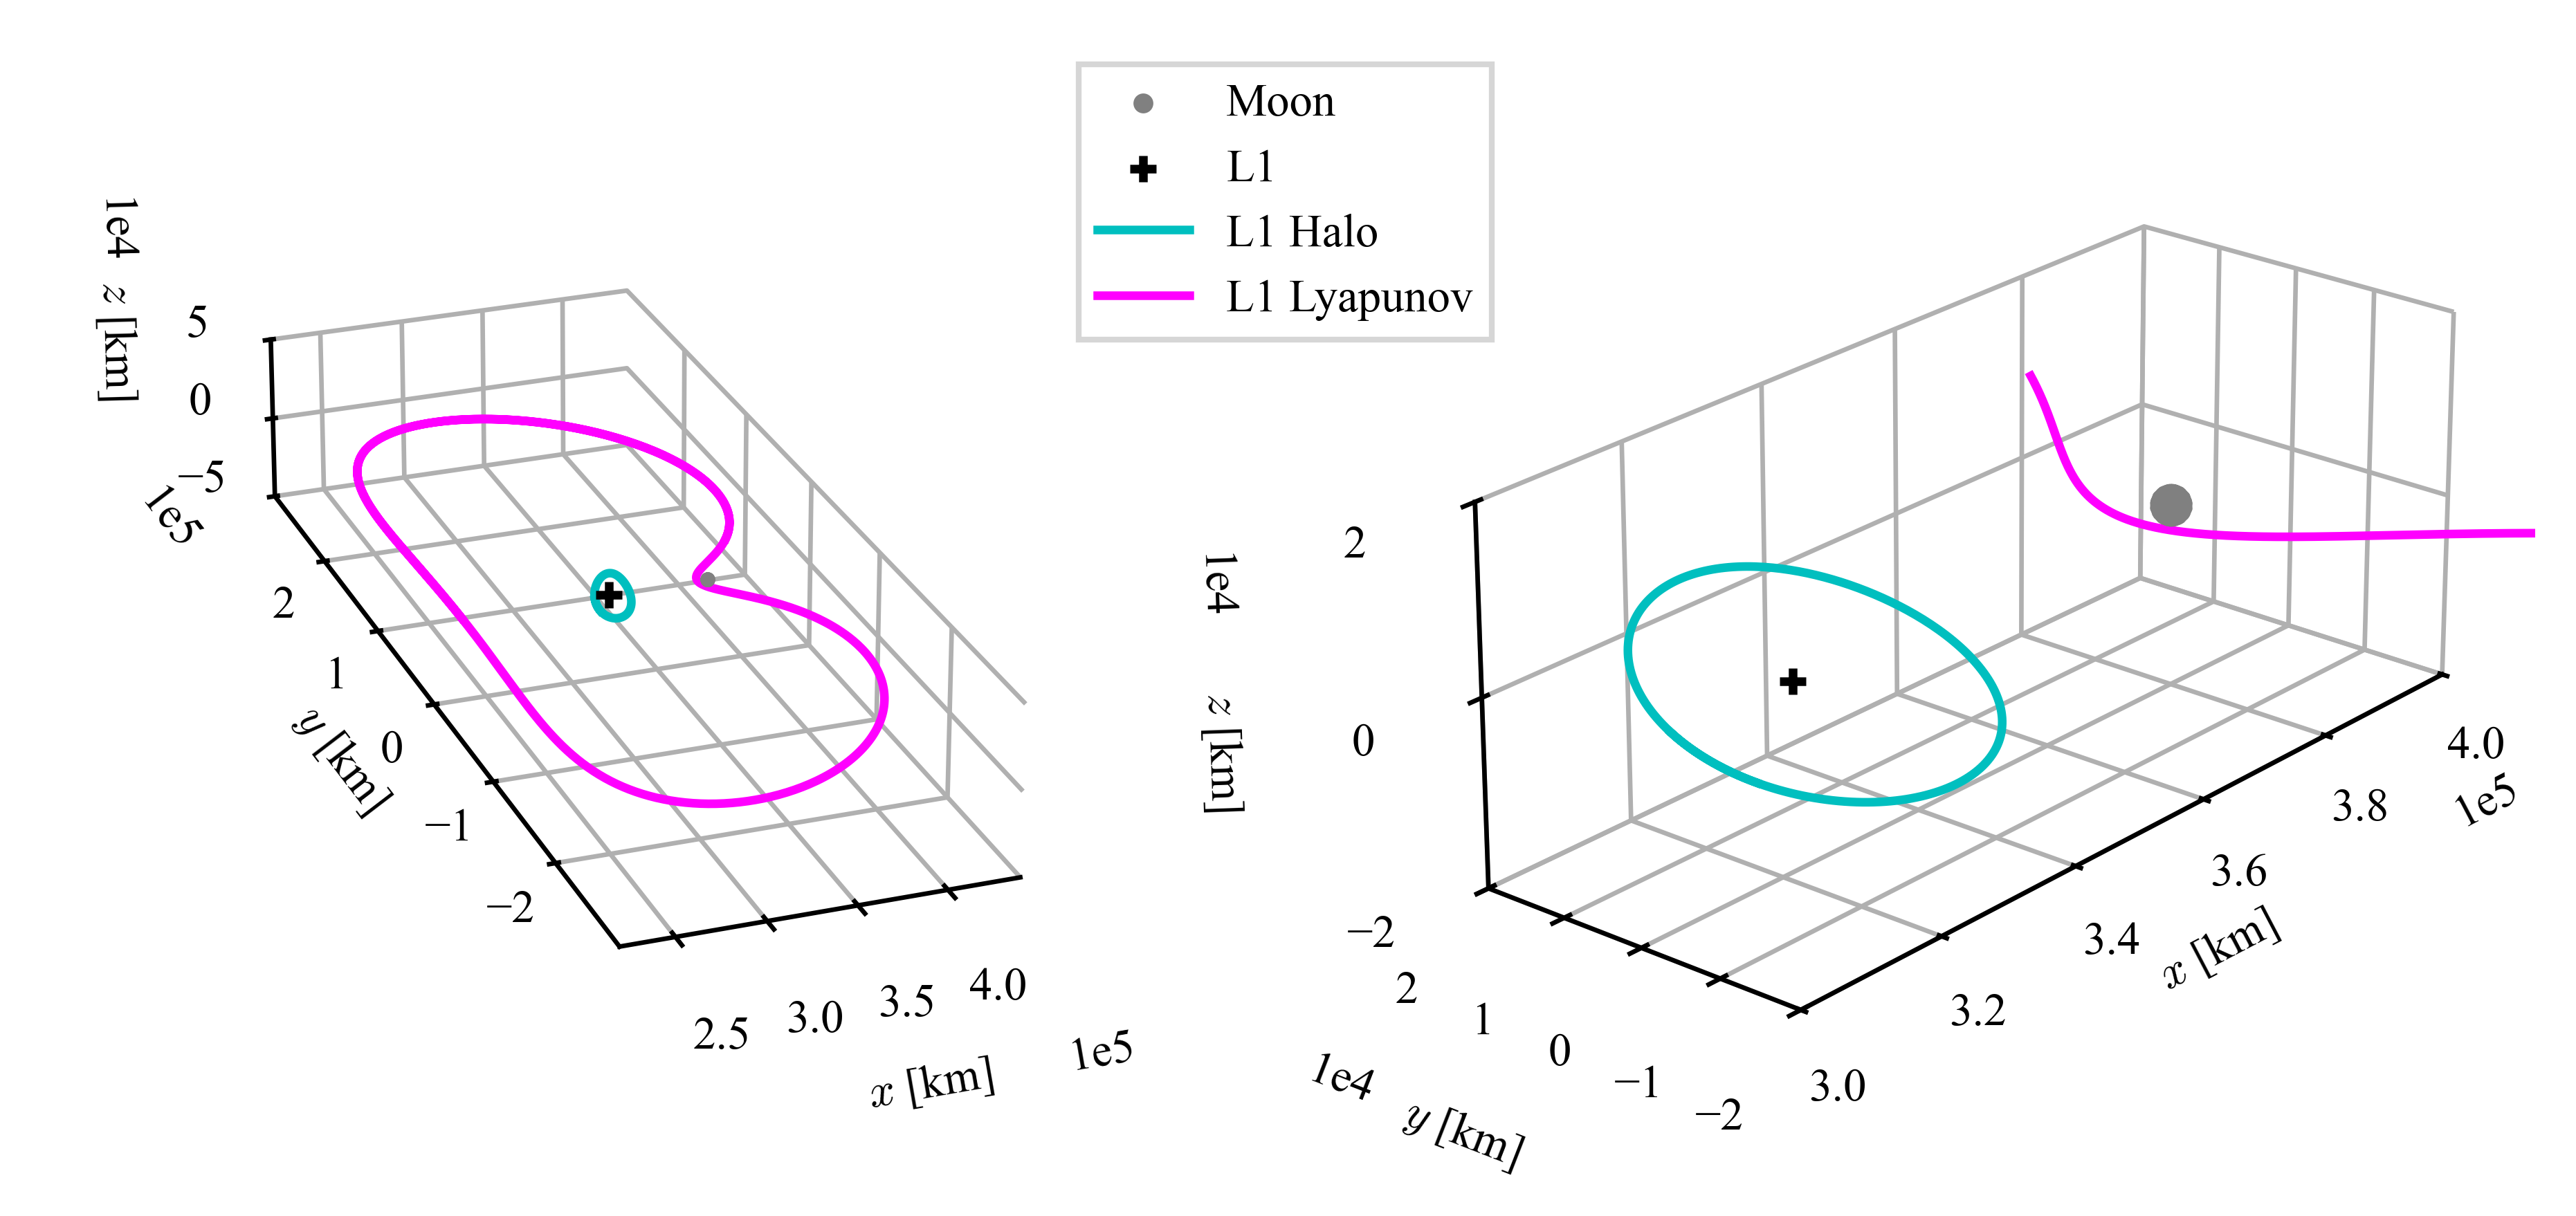
\includegraphics[width=0.85\linewidth]{Figures/orbits.png}
    \caption{Representative L1 Lyapunov and L1 Halo Periodic Orbits}
    \label{fig:orbits}
\end{figure}

It is desirable to obtain periodic solutions $\bm{\gamma}$ to the CR3BP dynamics (Eq. \ref{eq:CR3BP-dynamics}), such that
\begin{align}
    \bm{\gamma}(t + T) = \bm{\gamma}(t)
\end{align}
\noindent where $T$ is the period of the solution. These periodic orbits enable geometries impossible when only considering a single body's gravity. However, the dynamics of the CR3BP (Eq. \ref{eq:CR3BP-dynamics}) have no analytical closed-form solution, so these orbits are typically obtained using numerical methods.

Once a periodic solution has been obtained, continuation strategies can be employed to obtain a family of similar solutions \cite{williams2024dynamics}. The orbits of interest in this paper are those belonging to the L1 Lyapunov and L1 Halo families. These families are associated with the L1 Lagrange point, with the L1 Lyapunov family lying in the xy-plane and the L1 Halo family being three dimensional. These solutions are unstable, increasing the difficulty of the tracking problem, as small estimation errors caused by perturbations or maneuvers quickly expand during periods without observations. The representative orbits of interest are plotted in Figure \ref{fig:orbits}.

\subsection{Extended Kalman Filter (EKF)}

The ubiquitous Extended Kalman Filter (EKF) is an recursive estimation algorithm for systems with nonlinear dynamics/measurements \cite{smith1962application}. One iteration of the continuous-discrete EKF consists of two steps: a continuous time update and a discrete measurement update.

\begin{enumerate}
    \item Time Update
    
    The time update propagates the posterior estimate ${}^+\hat{\bm{x}}_{k-1}$ and estimation error covariance ${}^+P_{k-1}$ at the time of the previous measurement $t_{k-1}$ to the time of the current measurement $t_k$. The state is propagated with the nonlinear dynamics equation $\dot{\bm{x}} = \bm{f}(\bm{x})$, and the covariance is propagated with the state transition matrix $\Phi(t_k, t_{k-1})$ and process noise covariance $Q_{k-1}$, yielding the prior estimate and covariance at the current time, ${}^-\bm{\hat{x}}_k$ and ${}^-P_k$:
    \begin{align}
        {}^-\hat{\bm{x}}_k &= \int_{t_{k-1}}^{t_k} \bm{f}(\bm{\hat{x}}(t)) dt, & \hat{\bm{x}}(t_{k-1}) = {}^+\hat{\bm{x}}_{k-1} \label{nonlinear estimate propagation (first EKF equation)} \\
        {}^-P_k &= \Phi(t_k, t_{k-1}) {}^+P_{k-1} \Phi^\top(t_k, t_{k-1}) + Q_{k-1}\\
        \Phi(t_k, t_{k-1}) &= \int_{t_{k-1}}^{t_k} F(\hat{\bm{x}}(\tau))\Phi(\tau, t_{k-1}) d\tau, & \Phi(t_{k-1}, t_{k-1}) = I_{n\times n} \label{eq:STM-propagation}
    \end{align}
    Additionally, the nonlinear measurement equation $\bm{z} = \bm{h}(\bm{x})$ is applied to the prior estimate ${}^-\hat{\bm{x}}_k$ to obtain the predicted measurement, $\bm{\hat{z}}_k$.
    \begin{align}
        \bm{\hat{z}}_k = \bm{h}_k(\bm{\hat{x}}_k^-) \label{eq:predicted measurement}
    \end{align}

    \item Measurement Update
    
    After the time update, ${}^-\bm{\hat{x}}_k$ and ${}^-P_k$ are updated with the new measurement $\bm{z}_k = \bm{h}_k(\bm{x}_k) + \bm{w}_k$ to obtain the posterior estimate and covariance, ${}^-\bm{x}_k$ and ${}^+P_k$. Mathematically,
    \begin{align}
        ^+\bm{\hat{x}}_k &= K_k (\bm{z}_k - \bm{\hat{z}}_k) \label{eq:posterior-estimate-update}\\
        ^+P_k &= {}^-P_k - C_k K_k^\top - K_k C_k ^\top + K_k W_k K_k^\top \\
        K_k &= C_k W_k^{-1} \\
        C_k &= {}^-P_k H_k^\top({}^-\bm{\hat{x}}_k) \\
        W_k &= H_k^\top({}^-\bm{\hat{x}}_k) {}^-P_k H_k^\top({}^-\bm{\hat{x}}_k) + R_k \label{eq:innovations covariance (last EKF eq)}
    \end{align}
    \noindent where $K_k$ is the Kalman gain matrix, $C_k$ is the cross covariance matrix, $W_k$ is the innovations covariance matrix, $H_k({}^-\bm{\hat{x}}_k) = \partial \bm{h}({}^-\hat{\bm{x}}_k)/\partial\bm{x}$ is the measurement Jacobian, and $R_k = \E[\bm{w}_k\bm{w}_k^\top]$ is the measurement noise covariance.

\end{enumerate}

At the completion of the measurement update, one iteration of the EKF is completed, and the next iteration begins after setting $ t_k \rightarrow t_{k-1}$. 

\subsection{Interacting Multiple Model (IMM) Estimator}

The interacting multiple model (IMM) estimator is well-suited for tracking maneuvering targets because of its ability to incorporate multiple dynamics models into a single filter \cite{blom1988interacting,bar1989tracking,genovese2001interacting}. These different dynamics models can capture the discrete ``modes" of a maneuvering target which yields a more accurate estimate. 

Mathematically, the IMM assumes that the target's mode $\tau_k$ at time $t_k$ is one of $s$ discrete modes in the set of all modes $M = \{1, \cdots, s\}$, such that $\tau_k \in M $. Each mode $j \in M$ is associated with a dynamics model $\dot{\bm{x}} = \bm{f}^{(j)}(\bm{x})$, process noise covariance $Q^{(j)}$, posterior state estimate ${}^+\hat{\bm{x}}_k^{(j)}$, posterior estimate error covariance ${}^+P_k^{(j)}$, and mode probability $\mu^{(j)}_k = \P{\tau_k = j}$. The time evolution of these modes are modeled as a discrete-time Markov chain with associated row-stochastic transition matrix $\Pi \in \R_{s \times s}$, where element $\Pi_{i, j} = \P{\tau_k=j | \tau_{k-1} = i}$ .

One iteration of the IMM consists of three steps: probabilistic mixing, mode-dependent filtering, and mode probability update.

\begin{enumerate}
    \item Probabilistic Mixing

    The posterior state estimates ${}^+\hat{\bm{x}}_{k-1}^{(j)}$ and covariances ${}^+P_{k-1}^{(j)}$ are probabilistically combined to create mode-matched initial conditions for the mode-dependent filtering in the following step. The mode-matched estimate and covariance for each mode $j$ is denoted as ${}^{+}\hat{\bm{x}}_{k-1}^{0j}$ and ${}^+P_{k-1}^{0j}$, respectively, and are obtained with
    \begin{align}
        {}^+\hat{\bm{x}}_{k-1}^{0j} &= \sum_{i=1}^r {}^+\hat{\bm{x}}_{k-1}^{(i)} \mu_{k-1}^{i|j} \label{eq:mixed-initial-mean}\\
        {}^+P_{k-1}^{0j} &= \sum_{i=1}^r  \mu_{k-1}^{i|j} [{}^+P_{k-1}^{(i)} + ({}^+\bm{\hat{x}}_{k-1}^{(i)} - {}^+\bm{\hat{x}}_{k-1}^{0j})({}^+\bm{\hat{x}}_{k-1}^{(i)} - {}^+\bm{\hat{x}}_{k-1}^{0j})^\top ] \label{eq:mixed-initial-covariance}
    \end{align}
    \noindent where $\mu_k^{i|j}$ is the mixing probability, which captures how much of mode $i$'s posterior estimate should be mixed into mode $j$'s initial conditions. The mixing probabilities $\mu_k^{i|j}$ are computed as
    \begin{align}
        \mu_{k-1}^{i|j} &= \frac{1}{\bar{c}_{k-1}^{(j)}} \Pi_{i,j} \mu_{k-1}^{(i)} \\
        \bar{c}_{k-1}^{(j)} &= \sum_{i=1}^r \Pi_{i,j} \mu_{k-1}^{(i)} \label{mixing probability constant}
    \end{align}
    \noindent where $\bar{c}_{k-1}^{(j)}$ is a normalization constant such that $\sum_{i=1}^r \mu_{k-1}^{i|j} = 1$.
    
    \item Mode-Dependent Filtering

    After constructing the mode-matched initial conditions, an iteration of the EKF is performed for each mode $j \in M$ with Eqs. \ref{nonlinear estimate propagation (first EKF equation)}-\ref{eq:innovations covariance (last EKF eq)}, each with its own mode-matched initial conditions ${}^+\bm{\hat{x}}_{k-1}^{0j}$ and ${}^+P_{k-1}^{0j}$, dynamics equation $\bm{f}^{(j)}(\bm{x})$, and process noise covariance $Q^{(j)}$. This yields the posterior estimates and covariances for each mode ${}^+\hat{\bm{x}}_k^{(j)}$ and ${}^+P_k^{(j)}$.

    \item Mode Probability Update

    In addition to obtaining ${}^+\hat{\bm{x}}_k^{(j)}$ and ${}^+P_k^{(j)}$, the mode probabilities are updated according to the innovations likelihoods $\Lambda_k^{(j)}$ given by
    \begin{align}
        \Lambda_k^{(j)} = \dfrac{1}{\sqrt{|2\pi W_k^{(j)}|}} \exp[-\frac{1}{2} (\bm{z}_k - \bm{\hat{z}}_k^{(j)})^\top (W_k^{(j)})^{-1} (\bm{z}_k - \bm{\hat{z}}_k^{(j)})] \label{eq:innovations-likelihoods}
    \end{align}
    where $W_k^{(j)}$ is mode $j$'s innovations covariance defined in Eq. \ref{eq:innovations covariance (last EKF eq)}, and $\hat{\bm{z}}_k^{(j)}$ is mode $j$'s predicted measurement defined in Eq. \ref{eq:predicted measurement}. The mode probability update is 
    \begin{align}
    \mu_k^{(j)} & = \frac{1}{c_k} \Lambda_k^{(j)} \bar{c}_{k-1}^{(j)} \label{eq:mode-probability-update} \\
    c_k &= \sum_{i=1}^r \Lambda_k^{(i)} \bar{c}_{k-1}^{(i)} 
    \end{align}
    where $\bar{c}_{k-1}^{(j)}$ is defined in Eq. \ref{mixing probability constant} and $c_k$ is a normalization constant such that $\sum_{j=1}^r \mu_k^{(j)} = 1$. The computation of the mode probabilities concludes a single iteration of the IMM, and the next iteration begins after setting $t_k \rightarrow t_{k-1}$.

    \item Output

    To obtain a single output value for the posterior estimate ${}^+\hat{\bm{x}}_k$ and posterior covariance ${}^+P_k $, the various posterior estimates ${}^+\hat{\bm{x}}_k^{(j)}$ and covariances ${}^+P_k^{(j)}$ are combined using their mode probabilities $\mu_k^{(j)}$:
    \begin{align}
        {}^+\bm{\hat{x}}_k &= \sum_{j=1}^r \mu_k^{(j)} {}^+\bm{\hat{x}}_k^{(j)}  \\
        {}^+P_k &= \sum_{j=1}^r \mu_k^j [{}^+P_k^{(j)} + ({}^+\bm{\hat{x}}_k^{(j)} - {}^+\bm{\hat{x}}_k)({}^+\bm{\hat{x}}_k^{(j)} - {}^+\bm{\hat{x}}_k)^\top]
    \end{align}
    Note that computing these values is not necessary to iterate the IMM and is purely for output purposes.
    
\end{enumerate}


\subsection{Pontryagin's Minimum Principle}

A generic optimal control problem can be defined as
\begin{align}
\begin{split}
     \min_{\bm{x}(t), \bm{u}(t)} & \quad J = \int_{t_0}^{t_f} L(t, \bm{x}(t), \bm{u}(t)) dt \\
     \text{s.t.} & \quad  \dot{\bm{x}} = \bm{f}(t, \bm{x}, \bm{u}) \\
     & \quad \bm{\psi}(\bm{x}_0, \bm{x}_f, t_0, t_f) = \bm{0}
\end{split}
\end{align}
\noindent where $J$ is the cost to be minimized, $L$ is the Lagrangian cost, $\bm{f}$ is the dynamics equation, and $\bm{\psi}$ is the vector of boundary conditions. To obtain the conditions for optimality, we utilize Pontryagin's Minimum Principle (PMP), which states that the optimal control $\bm{u}^*(t)$ is given by
\begin{align}
    \bm{u}^*(t) = \argmin_{\bm{u}(t)} H(t, \bm{x}^*(t), \bm{u}(t), \bm{\lambda}(t)) \label{PMP optimal control}
\end{align}
\noindent where $H$ is the control Hamiltonian, defined as
\begin{align}
    H(t, \bm{x}(t), \bm{u}(t), \bm{\lambda}(t)) = L + \bm{\lambda}^\top \bm{f}(\bm{x}, \bm{u}) \label{PMP Hamiltonian}
\end{align}
\noindent and $\bm{\lambda} \in \R^{\text{dim}(\bm{x})}$ is the costate \cite{pontryagin1962}. The costate is governed by its own dynamics, given by
\begin{equation}
    \dot{\bm{\lambda}} = -\left(\frac{\partial H}{\partial\bm{x}} \right)^\top \label{PMP costate dynamics}
\end{equation}
Using PMP, optimality can be defined mathematically as a system of dynamical equations with the augmented state $\bm{x} = [\bm{\xi}^\top, \bm{\lambda}^\top]^\top$ for use in a sequential filtering algorithm, such as the IMM.

\section{Methodology}

\subsection{Pontryagin's Minimum Principle in the CR3BP}

\subsubsection{Minimum-Fuel}

We will first consider the minimum-fuel cost function, where the objective is to minimize the integral of the control norm $\norm{\bm{u}}_2$ over the trajectory. The minimum-fuel Lagrangian and control Hamiltonian $L_{MF}$ and $H_{MF}$ are then
\begin{align}
    L_{MF} &= \norm{\bm{u}}_2 \\
    H_{MF} &= \norm{\bm{u}}_2 + \bm{\lambda}^\top (\bm{g}(\bm{\xi}) + B\bm{u})
\end{align}
To apply the control optimality condition (Eq. \ref{PMP optimal control}), we rewrite the Hamiltonian $H_{MF}$ in terms of the primer vector $\bm{p} = B^\top \bm{\lambda}$. The rewritten Hamiltonian $H_{MF}$ is then
\begin{equation}
    H_{MF} = \norm{\bm{u}}_2 + \bm{u}^\top \bm{p} + \bm{\lambda}^\top \bm{g}(\bm{\xi})
\end{equation}
After rewriting $H_{MF}$ with $\bm{p}$, it is seen that $H_{MF}$ is minimized when $\bm{u}$ has its largest admissible magnitude and is antiparallel to $\bm{p}$, but only when $\norm{\bm{p}}_2 > 1$ \cite{lawden1963optimal}. When $\norm{\bm{p}}_2 < 1$, $H_{MF}$ is minimized when $\bm{u} = \bm{0}$. The resulting optimal control is then
\begin{equation}
    \bm{u}_{MF}^* = \Gamma^*_0 \hat{\bm{u}}^*, \quad \Gamma^*_0 = \begin{cases}
        u_{\text{max}}, & \norm{\bm{p}}_2 > 1 \\
        0, & \norm{\bm{p}}_2 < 1
    \end{cases}, \quad \hat{\bm{u}}^* = -\frac{\bm{p}}{\norm{\bm{p}}_2}, \quad \bm{p} = B^\top \bm{\lambda} \label{eq:min-fuel control}
\end{equation}
Note that the resulting optimal control is "bang-bang," requiring instantaneous switching between maximum and minimum control magnitudes. To avoid the numerical difficulties in applying this control directly, the optimal control is approximated with a hyperbolic tangent smoothing function:  
\begin{equation}
    \Gamma^* = \frac{u_{\text{max}}}{2} \left[1 + \tanh \left(\frac{\norm{\bm{p}}_2 - 1}{\rho} \right)\right] \approx \Gamma_0^* \label{hyperbolic tangent smoothing}
\end{equation}
\noindent where $\rho$ is a smoothing parameter such that $\lim_{\rho \rightarrow 0} \Gamma^* = \Gamma_0^*$ \cite{taheri2018generic, junkins2019exploration}.

Applying the necessary condition for the costate dynamics in Eq. \ref{PMP costate dynamics} yields
\begin{equation}
    \dot{\bm{\lambda}}_{MF}^* = -G(\bm{\xi})^\top \bm{\lambda} \label{eq:min-fuel-costate-dynamics}
\end{equation}
\noindent where $G(\bm{\xi}) = \partial \bm{g}(\bm{\xi})/\partial \bm{\xi}$ is the Jacobian matrix of the ballistic CR3BP dynamics.

\subsubsection{Minimum-Time}

We will now consider the minimum-time optimal control problem. The Lagrangian and control Hamiltonian $L_{MT}$ and $H_{MT}$ are then
\begin{align}
    L_{MT} &= 1 \\
    H_{MT} &= 1 + \bm{\lambda}^\top (\bm{g}(\bm{\xi}) + B\bm{u})
\end{align}
To apply the control optimality condition (Eq. \ref{PMP optimal control}), we rewrite the Hamiltonian with the primer vector $\bm{p} = B^\top \bm{\lambda}$. The rewritten Hamiltonian $H_{MT}$ is then
\begin{align}
    H_{MT} = 1 + \bm{u}^\top \bm{p}
\end{align}
Now considering $H_{MT}$ formulated with the primer vector $\bm{p}$, $H_{MT}$ is minimized when $\bm{u}$ has its largest admissible magnitude and is antiparallel to $\bm{p}$. The resulting optimal control is then
\begin{align}
    \bm{u}_{MT}^* = - u_\text{max}\hat{\bm{u}}^*, \quad \hat{\bm{u}}^* = -\frac{\bm{p}}{\norm{\bm{p}}_2}, \quad \bm{p} = B^\top \bm{\lambda} \label{eq:min-time-control}
\end{align}
Note that $\bm{u}_{MT}^* = \bm{u}_{MF}^*$ when $\norm{\bm{p}}_2 > 1$. This will be the justification for modeling minimum-fuel optimal control as minimum-time optimal control in the filtering implementation.

Applying the necessary condition for the costate dynamics given in Eq. \ref{PMP costate dynamics} yields
\begin{equation}
    \dot{\bm{\lambda}}_{MT}^* = -G(\bm{\xi})^\top \bm{\lambda} \label{eq:min-time-costate-dynamics}
\end{equation}
\noindent where $G(\bm{\xi}) = \partial \bm{g}(\bm{\xi})/\partial \bm{\xi}$ is the Jacobian matrix of the natural CR3BP dynamics. Note that the expression for $\dot{\bm{\lambda}}_{MT}^*$ (Eq. \ref{eq:min-time-costate-dynamics}) is identical to the expression for $\dot{\bm{\lambda}}_{MF}^*$ (Eq. \ref{eq:min-fuel-costate-dynamics}).


\subsection{Optimal Control IMM (OCIMM)}

To track maneuvering low-thrust spacecraft in cislunar space, we utilize an IMM with two modes: a coasting mode ($\tau=1$) and a maneuvering mode ($\tau=2$). The state vector of the estimator includes the original CR3BP state as well as the costate, written as $\bm{x} = [\bm{\xi}^\top, \bm{\lambda}^\top]^\top \in \R^{12}$. The costate can further be subdivided to be written as $\bm{\lambda} = [\bm{\lambda}_r^\top, \bm{\lambda}_v^\top]^\top$, where $\bm{\lambda}_r \in \R^3$ and $\bm{\lambda}_v \in \R^3$ are the vectors of costates corresponding to the vectors of states $\bm{r}$ and $\bm{v}$, respectively. The dynamics of the maneuvering mode are a spacecraft operating under an assumed minimum-time optimal control policy:
\begin{align}
    \bm{f}^{(2)}(\bm{x}) &= \begin{bmatrix}
        \dot{\bm{\xi}} \\
        \dot{\bm{\lambda}}
    \end{bmatrix} = \begin{bmatrix}
        \bm{g}(\bm{\xi}) + B \bm{u}^*_{MT} \\
        -G(\bm{\xi})^\top \bm{\lambda}
    \end{bmatrix}
\end{align}
The justification behind assuming time-optimal dynamics is that the costates during a thrusting arc of a fuel-optimal control policy would produce an identical control profile under a time-optimal control policy. This is known by comparing the expressions for $\bm{u}^*_{MF}$ and $\dot{\bm{\lambda}}_{MF}^*$ (Eqs. \ref{eq:min-fuel control}, \ref{eq:min-fuel-costate-dynamics}) with the expressions for $\bm{u}^*_{MT}$ and $\dot{\bm{\lambda}}_{MT}^*$ (Eqs. \ref{eq:min-time-control}, \ref{eq:min-time-costate-dynamics}). While it is possible to directly implement an assumed fuel-optimal control policy into the OCIMM, the extreme nonlinearity resulting from the bang-bang control (even with hyperbolic tangent smoothing given in Eq. \ref{hyperbolic tangent smoothing}) causes divergence problems when used in a sequential filter, as observed from numerical experiments. Further research to enable direct implementation of assumed minimum-fuel control may prove beneficial for improved trajectory prediction, even in the presence of extended observation gaps. 

The coasting mode ($\tau=1$) has assumed ballistic CR3BP dynamics for the state, and the same time-optimal dynamics for the costate:
\begin{align}
    \bm{f}^{(1)}(\bm{x}) &= \begin{bmatrix}
        \dot{\bm{\xi}} \\
        \dot{\bm{\lambda}}
    \end{bmatrix} = \begin{bmatrix}
        \bm{g}(\bm{\xi}) \\
        -G(\bm{\xi})^\top \bm{\lambda}
    \end{bmatrix}\label{eq:OCIMM-coasting-dynamics}
\end{align}
\noindent By having the costate dynamics of the coasting mode be the same time-optimal costate dynamics, we can track the dynamics of a fuel-optimal trajectory with greater numerical stability. 

Consider a spacecraft maneuvering under a fuel-optimal trajectory. Since the costate dynamics of fuel-optimal and time-optimal trajectories are the same, the OCIMM's assumed time-optimal costate dynamics are precisely correct. However, the problem with tracking this spacecraft is its bang-bang control law. From the perspective of an outside observer attempting to discern $\bm{\lambda}$, the only information available would be the spacecraft's state and control inputs. From this information, even if highly accurate, it is extremely difficult to obtain $\bm{\lambda}$, as many costates can produce the same control. This is demonstrated by examining the fuel-optimal control law (Eq. \ref{eq:min-fuel control}). During periods of coasting, the only information known is that $\norm{\bm{\lambda}_v}_2 < 1$, and during periods of thrusting, the only information known is the direction of $\bm{\lambda}_v$ and that $\norm{\bm{\lambda}_v}_2 > 1$. Then, even assuming a decent estimate of $\bm{\lambda}$ can be obtained, a slight error could be the difference between thrusting and coasting for a filter assuming fuel-optimal control. The proposed solution is to use an IMM with two modes, where the control during the thrusting arcs is modeled using the more well-behaved time-optimal dynamics.

The key benefit of assuming optimal maneuvers is that given some observation of the beginning of a maneuver, it is possible to somewhat predict the rest of the maneuver. Thus, if an observation gap were to occur over the rest of the maneuver due to either natural causes (e.g. Moon occultation) or artificial causes (e.g. sensor re-tasking), the estimator can obtain a more accurate estimate. 

\subsection{Acceleration IMM}

For a baseline, we compare the performance of the OCIMM to an IMM with assumed third order dynamics, denoted as the ``acceleration IMM." The acceleration IMM has two modes: a coasting mode ($\tau = 1$) and a maneuvering mode ($\tau = 2$). The acceleration IMM estimates the control (acceleration) of the spacecraft $\bm{\eta}$ in addition to its position and velocity, such that its state vector is defined as $\bm{x}_a = [\bm{\xi}^\top, \bm{\eta}^\top]^\top$. The dynamics of the acceleration IMM are given in Eq. 
\begin{align}
    \bm{f}^{(1)}_a (\bm{x}_a) &= \begin{bmatrix}
        \dot{\bm{\xi}} \\
        \dot{\bm{\eta}}
    \end{bmatrix} = \begin{bmatrix}
        \bm{g}(\bm{\xi}) \\
        \bm{0}_{3 \times 1}
    \end{bmatrix} \label{eq:accel-IMM-coasting-dynamics} \\
    \bm{f}^{(2)}_a (\bm{x}_a) &= \begin{bmatrix}
        \dot{\bm{\xi}} \\
        \dot{\bm{\eta}}
    \end{bmatrix} = \begin{bmatrix}
        \bm{g}(\bm{\xi}) + B \bm{\eta} \\
        \bm{0}_{3 \times 1}
    \end{bmatrix} \label{eq:accel-IMM-thrusting-dynamics}
\end{align}

Notably, the dynamics of the acceleration IMM assume that the spacecraft's control is constant, i.e. $\dot{\bm{\eta}} = \bm{0}$. Therefore, the acceleration IMM is unable to predict how the control will evolve over time. This is the main advantage of the OCIMM over the acceleration IMM.

It should be noted that the the OCIMM requires an assumption of knowledge of $u_\text{max}$, while the acceleration IMM does not. However, the process noise covariance corresponding to the acceleration IMM's control estimate must be tuned, which is informed by general knowledge of the maximum thrust of the spacecraft. Thus, the acceleration IMM also requires some knowledge of $u_\text{max}$. 

\subsection{Observation Strategy}

Because of the difficulty of observing cislunar spacecraft from Earth, angles-only measurements are obtained from a constellation of $m$ observer spacecraft in a distant retrograde orbit at a frequency of once per hour \cite{gupta2023constellation}. It is assumed that the positions of the observer satellites are known deterministically. The azimuth and elevation measurements $\theta_k^{(i)}$ and $\phi_k^{(i)}$ from observer spacecraft $i \in [1, \cdots, m]$ at time $t_k$ are given by
\begin{align}
    \begin{bmatrix}
        \theta_k^{(i)} \\
        \phi_k^{(i)}
    \end{bmatrix} = \begin{bmatrix}
        \tan^{-1}\left(\frac{y_k - \bar{y}_k^{(i)}}{x_k - \bar{x}_k^{(i)}}\right) \\
        \tan^{-1}\left(\frac{z_k - \bar{z}_k^{(i)}}{\sqrt{(x_k - \bar{x}_k^{(i)})^2 + (y_k - \bar{y}_k^{(i)})^2}}\right)
    \end{bmatrix} + w_k^{(i)}
\end{align}
\noindent where $\bar{x}_k^{(i)}$, $\bar{y}_k^{(i)}$, and $\bar{z}_k^{(i)}$ are the respective $x$, $y$, and $z$ components of the observer spacecraft's position in the CR3BP coordinate frame, and $w_k^{(i)} \sim \mathcal{N}(0, \text{diag}(\sigma_\theta, \sigma_\phi))$ is Gaussian, zero-mean measurement noise. 

To improve estimation performance when using angles-only measurements, we implement the pointing vector reformulation developed by Craig and Oguri \cite{craig2024robust}. The general idea of the pointing vector reformulation is to transform the nonlinear angles-only measurement equation into a linear Cartesian measurement equation with a properly transformed measurement noise covariance matrix. The pointing vector measurement equation for a single sensor $i \in [1, \cdots, m]$ is then 
\begin{align}
    \bm{h}_k^{(i)}(\bm{x}_k) &= \begin{bmatrix}
        I_3 & 0_{3 \times 9}
    \end{bmatrix} \bm{x}_k - \bar{\bm{r}}_k^{(i)}
\end{align}
\noindent where $\bar{\bm{r}}_k^{(i)} = [\bar{x}_k^{(i)}, \bar{y}_k^{(i)}\bar{z}_k^{(i)}]^\top$ is the deterministically known position of observer spacecraft $i$ at time $t_k$. Implementation of the pointing vector measurement equation into the measurement update requires the measurement Jacobian $H_k^{(i)}$ and measurement noise covariance matrix $R_k^{(i)}$. These are given by
\begin{align}
    H_k^{(i)} &= \begin{bmatrix}
        I_3 & \bm{0}_{3 \times 9} 
    \end{bmatrix} \\
    R_k^{(i)} &= \sigma_\theta^2 \bm{v}_1^{(i)}\bm{v}_1^{(i)}\top + \sigma_\phi^2\bm{v}_2^{(i)}\bm{v}_2^{(i)\top} + \sigma_\text{scl}^2 \bar{\bm{Z}}_k^{(i)} \bar{\bm{Z}}_k^{(i)\top} \\
    \bm{v}_1^{(i)} &= \hat{r}_k^{(i)}\begin{bmatrix}
        -\cos \theta_k^{(i)} \sin \phi_k^{(i)} \\
        -\sin \theta_k^{(i)} \sin \phi_k^{(i)} \\
        \cos \phi_k^{(i)}
    \end{bmatrix}, \quad \bm{v}_2^{(i)} = \hat{r}_k^{(i)} \begin{bmatrix}
        \sin \theta_k^{(i)} \\
        -\cos \theta_k^{(i)} \\
        0
    \end{bmatrix} \notag \\
    \bar{\bm{Z}}_k^{(i)} &= \bm{h}_k^{(i)}({}^-\hat{\bm{x}}_k), \quad \hat{r}_k^{(i)} = \norm{\bar{\bm{Z}}_k^{(i)}}_2 \notag
\end{align}
The new measurement noise covariance transforms the uncertainty in the measurement angles to Cartesian space. The lack of range information in the radial direction is represented by $\sigma_\text{scl}$, which is some large uncertainty projected in the radial direction. 

The measurements of $m$ spacecraft at the same time $t_k$ are processed in the measurement update by constructing a combined measurement vector with associated measurement Jacobian and measurement noise covariance matrix. 
\begin{align}
\begin{aligned}
    \bm{z}_k &= \begin{bmatrix}
        \bm{z}_k^{(1)} \\
        \vdots \\
        \bm{z}_k^{(m)}
    \end{bmatrix}, \quad \hat{\bm{z}}_k = \begin{bmatrix}
        \hat{\bm{z}}_k^{(1)} \\
        \vdots \\
        \hat{\bm{z}}_k^{(m)}
    \end{bmatrix}, \quad H_k = \begin{bmatrix}
        I_3 & 0_{3\times9} \\
        \vdots & \vdots \\
        I_3 & 0_{3\times9}
    \end{bmatrix} \in \R^{3m \times 12} \\
    \quad R_k &= \text{blkdiag}(R_k^{(1)}, \cdots, R_k^{(m)})
\end{aligned}
\end{align}

\subsection{Observation Checks}

To simulate realistic observation conditions, we implement two types of observation condition checks: exclusion angles and Moon shadows. The exclusion angles check whether the line of sight from the sensor to the target spacecraft is too close to the line of sight to an astronomical body. The three astronomical bodies considered are the Earth, Sun, and Moon. Mathematically, the sensor is unable to obtain a measurement of the target spacecraft if $\psi_{E/M/S}^{(i)} < \psi_{E/M/S}^{\text{min}}$, where $\psi_{E/M/S}^{(i)}$ is the angle between sensor $i$'s line of sight vectors to the target spacecraft and the body, $\psi_{E/M/S}^{\text{min}}$ is the minimum allowed separation angle, and subscripts $E$, $M$, and $S$ correspond to the Earth, Moon, or Sun, respectively.

\subsection{Underweighting}

Since the dynamics of the OCIMM are highly nonlinear and the magnitude of $\bm{\lambda}$ is not well known, a common issue is that the costate error covariance reduces too quickly at the end of observation gaps due to highly accurate measurements. This causes the OCIMM to become overconfident and unresponsive to changes in control. To alleviate this issue, we apply underweighting which applies a smaller update when there is a large difference between the predicted measurement error covariance and the actual measurement error covariance \cite{craig2024robust}. Underweighting is applied when the following condition is met:
\begin{align}\label{eq:underweighting-check}
    \tr(H_k {}^-P_k H_k^\top) > \frac{p}{1 - p} \tr(R_k)
\end{align}
In the case when underweighting is applied, the innovations covariance (originally given by Eq. \ref{eq:innovations covariance (last EKF eq)}) is modified to take the form
\begin{align}\label{eq:underweighted-update}
    W_k = \frac{1}{p} H_k^\top({}^-\bm{\hat{x}}_k) {}^-P_k H_k^\top({}^-\bm{\hat{x}}_k) + R_k 
\end{align}
The rest of the measurement update proceeds as normal. Implementing underweighting allows the OCIMM to gradually adjust its estimate as new measurements are processed at the end of observation gaps. 

\section{Simulation}

To test the tracking performance of the OCIMM, we simulate the tracking of a low-thrust spacecraft maneuvering from an L1 halo orbit to an L1 Lyapunov orbit under a minimum-fuel control policy, detailed in Figure \ref{fig:truth_trajectory}. The justification for a minimum-fuel trajectory is that fuel is a finite resource for a spacecraft, so to conserve this finite resource a minimum-fuel control policy is a likely choice.

\begin{figure}
    \centering
    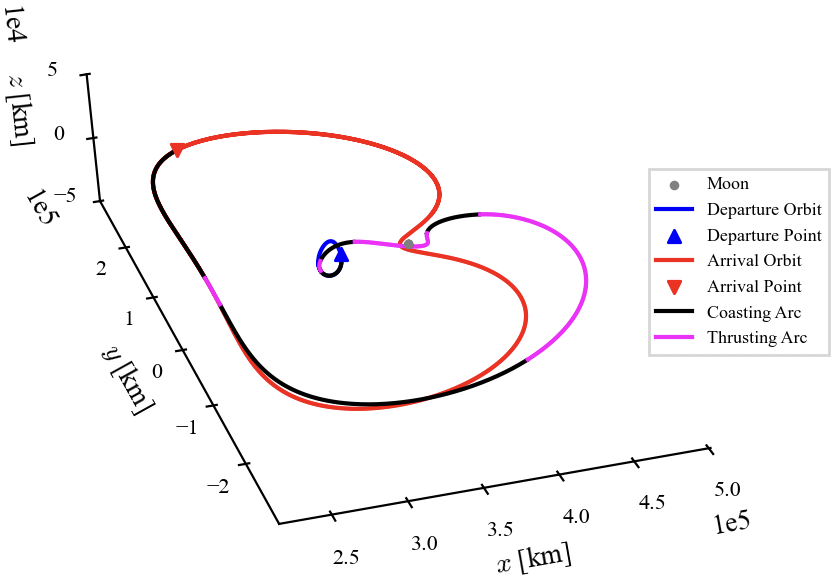
\includegraphics[width=\linewidth]{Figures/truth_trajectory.png}
    \caption{Truth transfer trajectory, with initial orbit, final orbit, coasting/thrusting arcs, observer orbit, observer initial positions, and truth control history.}
    \label{fig:truth_trajectory}
\end{figure}

We perform simulations for two scenarios: one with measurements available at all times, and another with all observation checks enforced to assess the ability of the OCIMM to predict control. Each scenario is ran with 100 Monte Carlo simulations, where each simulation differs in the initial state estimate ${}^+\hat{\bm{x}}_0$ and measurement noise values $\bm{w}_k^{(i)}$. The initial estimates for the state ${}^+\hat{\bm{\xi}}_0 \sim \mathcal{N}(\bm{\xi}(0), \text{blkdiag}(\sigma_{\bm{r}}I_3, \sigma_{\bm{v}}I_3))$ are drawn from a normal distribution with mean of the truth state and covariance of the initial state covariance. The estimates of the costates are initialized as ones, and the estimates of the acceleration IMM's control are initialized as zeros , such that $\bm{\lambda}_0 = \bm{1}_{6 \times 1}$ and $\bm{\eta}_0 = \bm{0}_{3\times1}$. The simulation parameters are listed in Table \ref{tab:truth-parameters}.

\begin{table}
    \centering
    \caption{Simulation parameters}
    \begin{tabular}{c|c}
        Parameter & Value \\
        \hline
        Smoothing Parameter, $\rho$, [n.d.] & $10^{-4}$ \\
        CR3BP Mass Ratio, $\mu$, [n.d.] & $1.215059\times 10^{-2}$ \\
        Max Control Acceleration, $u_\text{max, 0}$, [mm/s$^2$] & $0.4$ \\
        Measurement Angle S.D., $\sigma_\theta=\sigma_\phi$, [deg] & 0.001 \\
        Range Uncertainty, $\sigma_\text{scl}$, [n.d.] & 100 \\
        Iniital Mode Probabilities, $[\mu_0^{(1)}, \mu_0^{(2)}]$, [n.d.] & $[0.99, 0.01]$ \\
        Initial Position S.D., $\sigma_r(0)$, [km] & $50$ \\
        Initial Velocity S.D., $\sigma_v(0)$, [m/s] & 1 \\
        Initial Costate S.D., $\sigma_{\bm{\lambda}}(0)$, [n.d.] & 0.01  \\
        Initial Acceleration S.D., $\sigma_{\bm{\eta}}(0)$, [mm/s$^2$] & 1 \\
        Damping Ratio, $p$, [n.d.] & 0.5 \\
        Mode Transition Matrix, $\Pi$, [n.d.] & $\begin{bmatrix}
            0.99 & 0.01 \\
            0.01 & 0.99
        \end{bmatrix}$ \\
        OCIMM Coasting Process Noise, $Q^{(1)}$, [n.d.] & $\text{blkdiag}(10^{-30}I_6, 10^{-4}I_6)$ \\
        OCIMM Maneuvering Process Noise, $Q^{(2)}$, [n.d.] & $\text{blkdiag}(10^{-30}I_3, 10^{-18}I_3, 10^{-2}I_3, 10^{-4}I_3)$ \\
        Acceleration IMM Coasting Process Noise, $Q^{(1)}_a$, [n.d.] & $\text{blkdiag}(10^{-30}I_6, 10^{-4}I_3)$ \\
        Acceleration IMM Maneuvering Process Noise, $Q^{(2)}_a$, [n.d.] & $\text{blkdiag}(10^{-30}I_3, 10^{-18}I_3, 10^{-4}I_3)$
    \end{tabular}
    \label{tab:truth-parameters}
\end{table}

\section{Results}
\subsection{Fully-Observed Scenario}

\begin{figure}
    \centering
    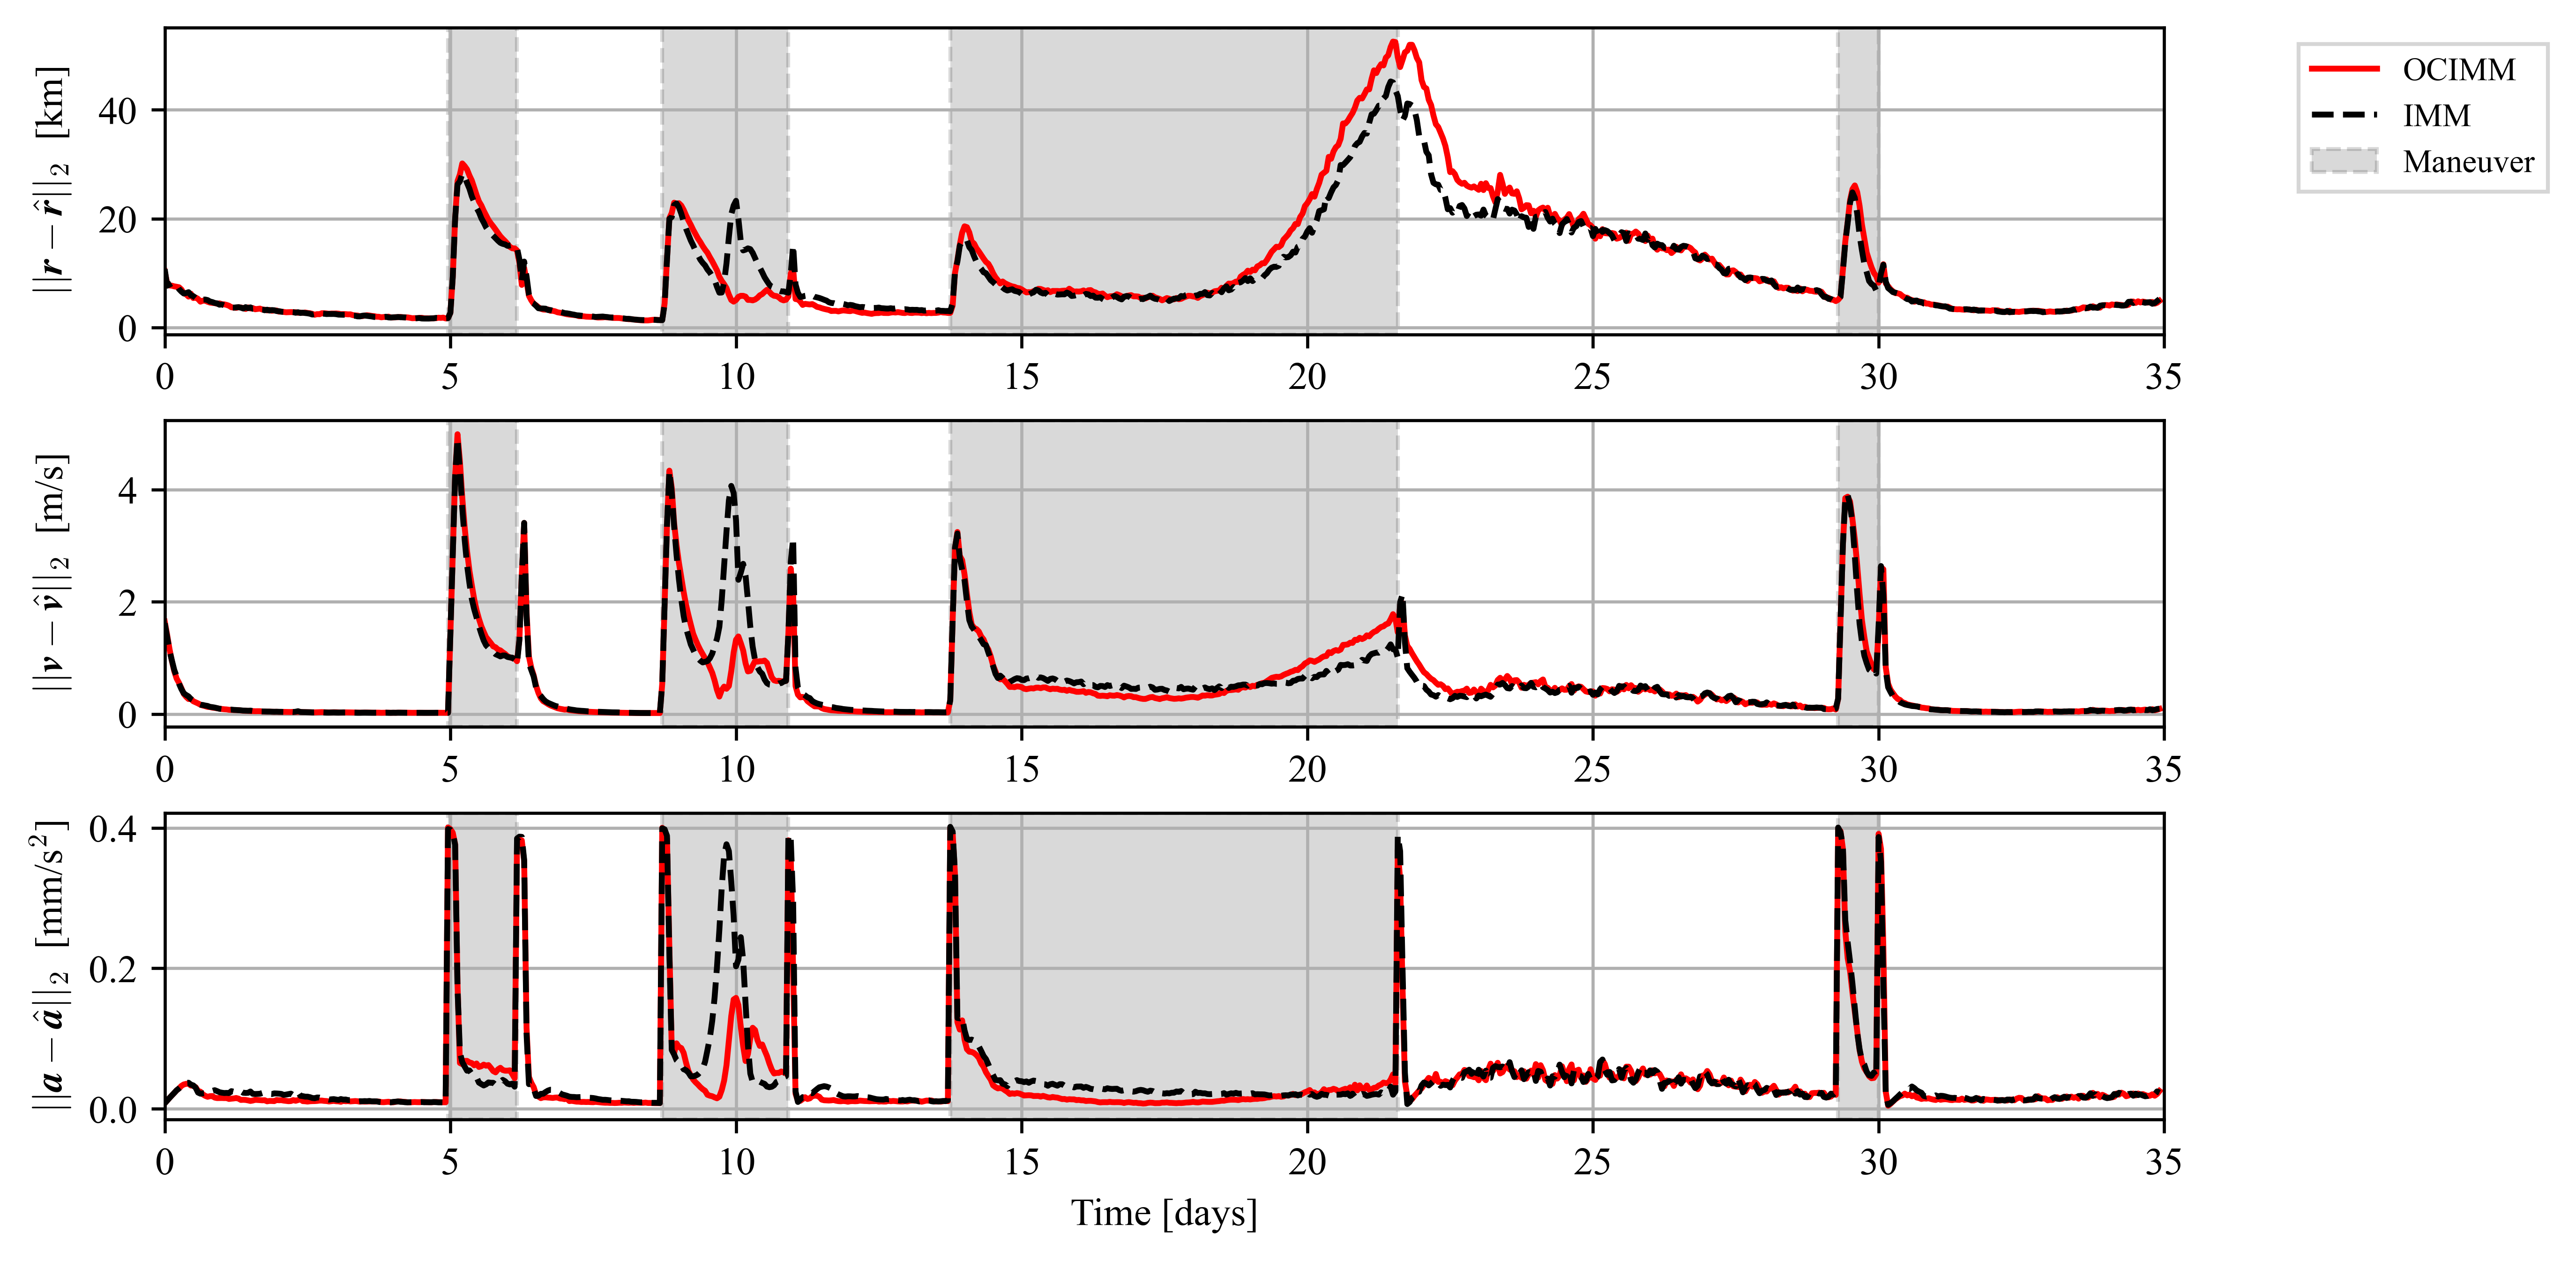
\includegraphics[width=1\linewidth]{Figures/MAE_normal.png}
    \caption{Mean absolute position, velocity, and acceleration estimation errors of acceleration IMM (black dashed lines) and OCIMM (red lines) for fully observed scenario. Grey shading indicates truth maneuvering periods.}
    \label{fig:MAE-normal}
\end{figure}

\begin{figure}
    \centering
    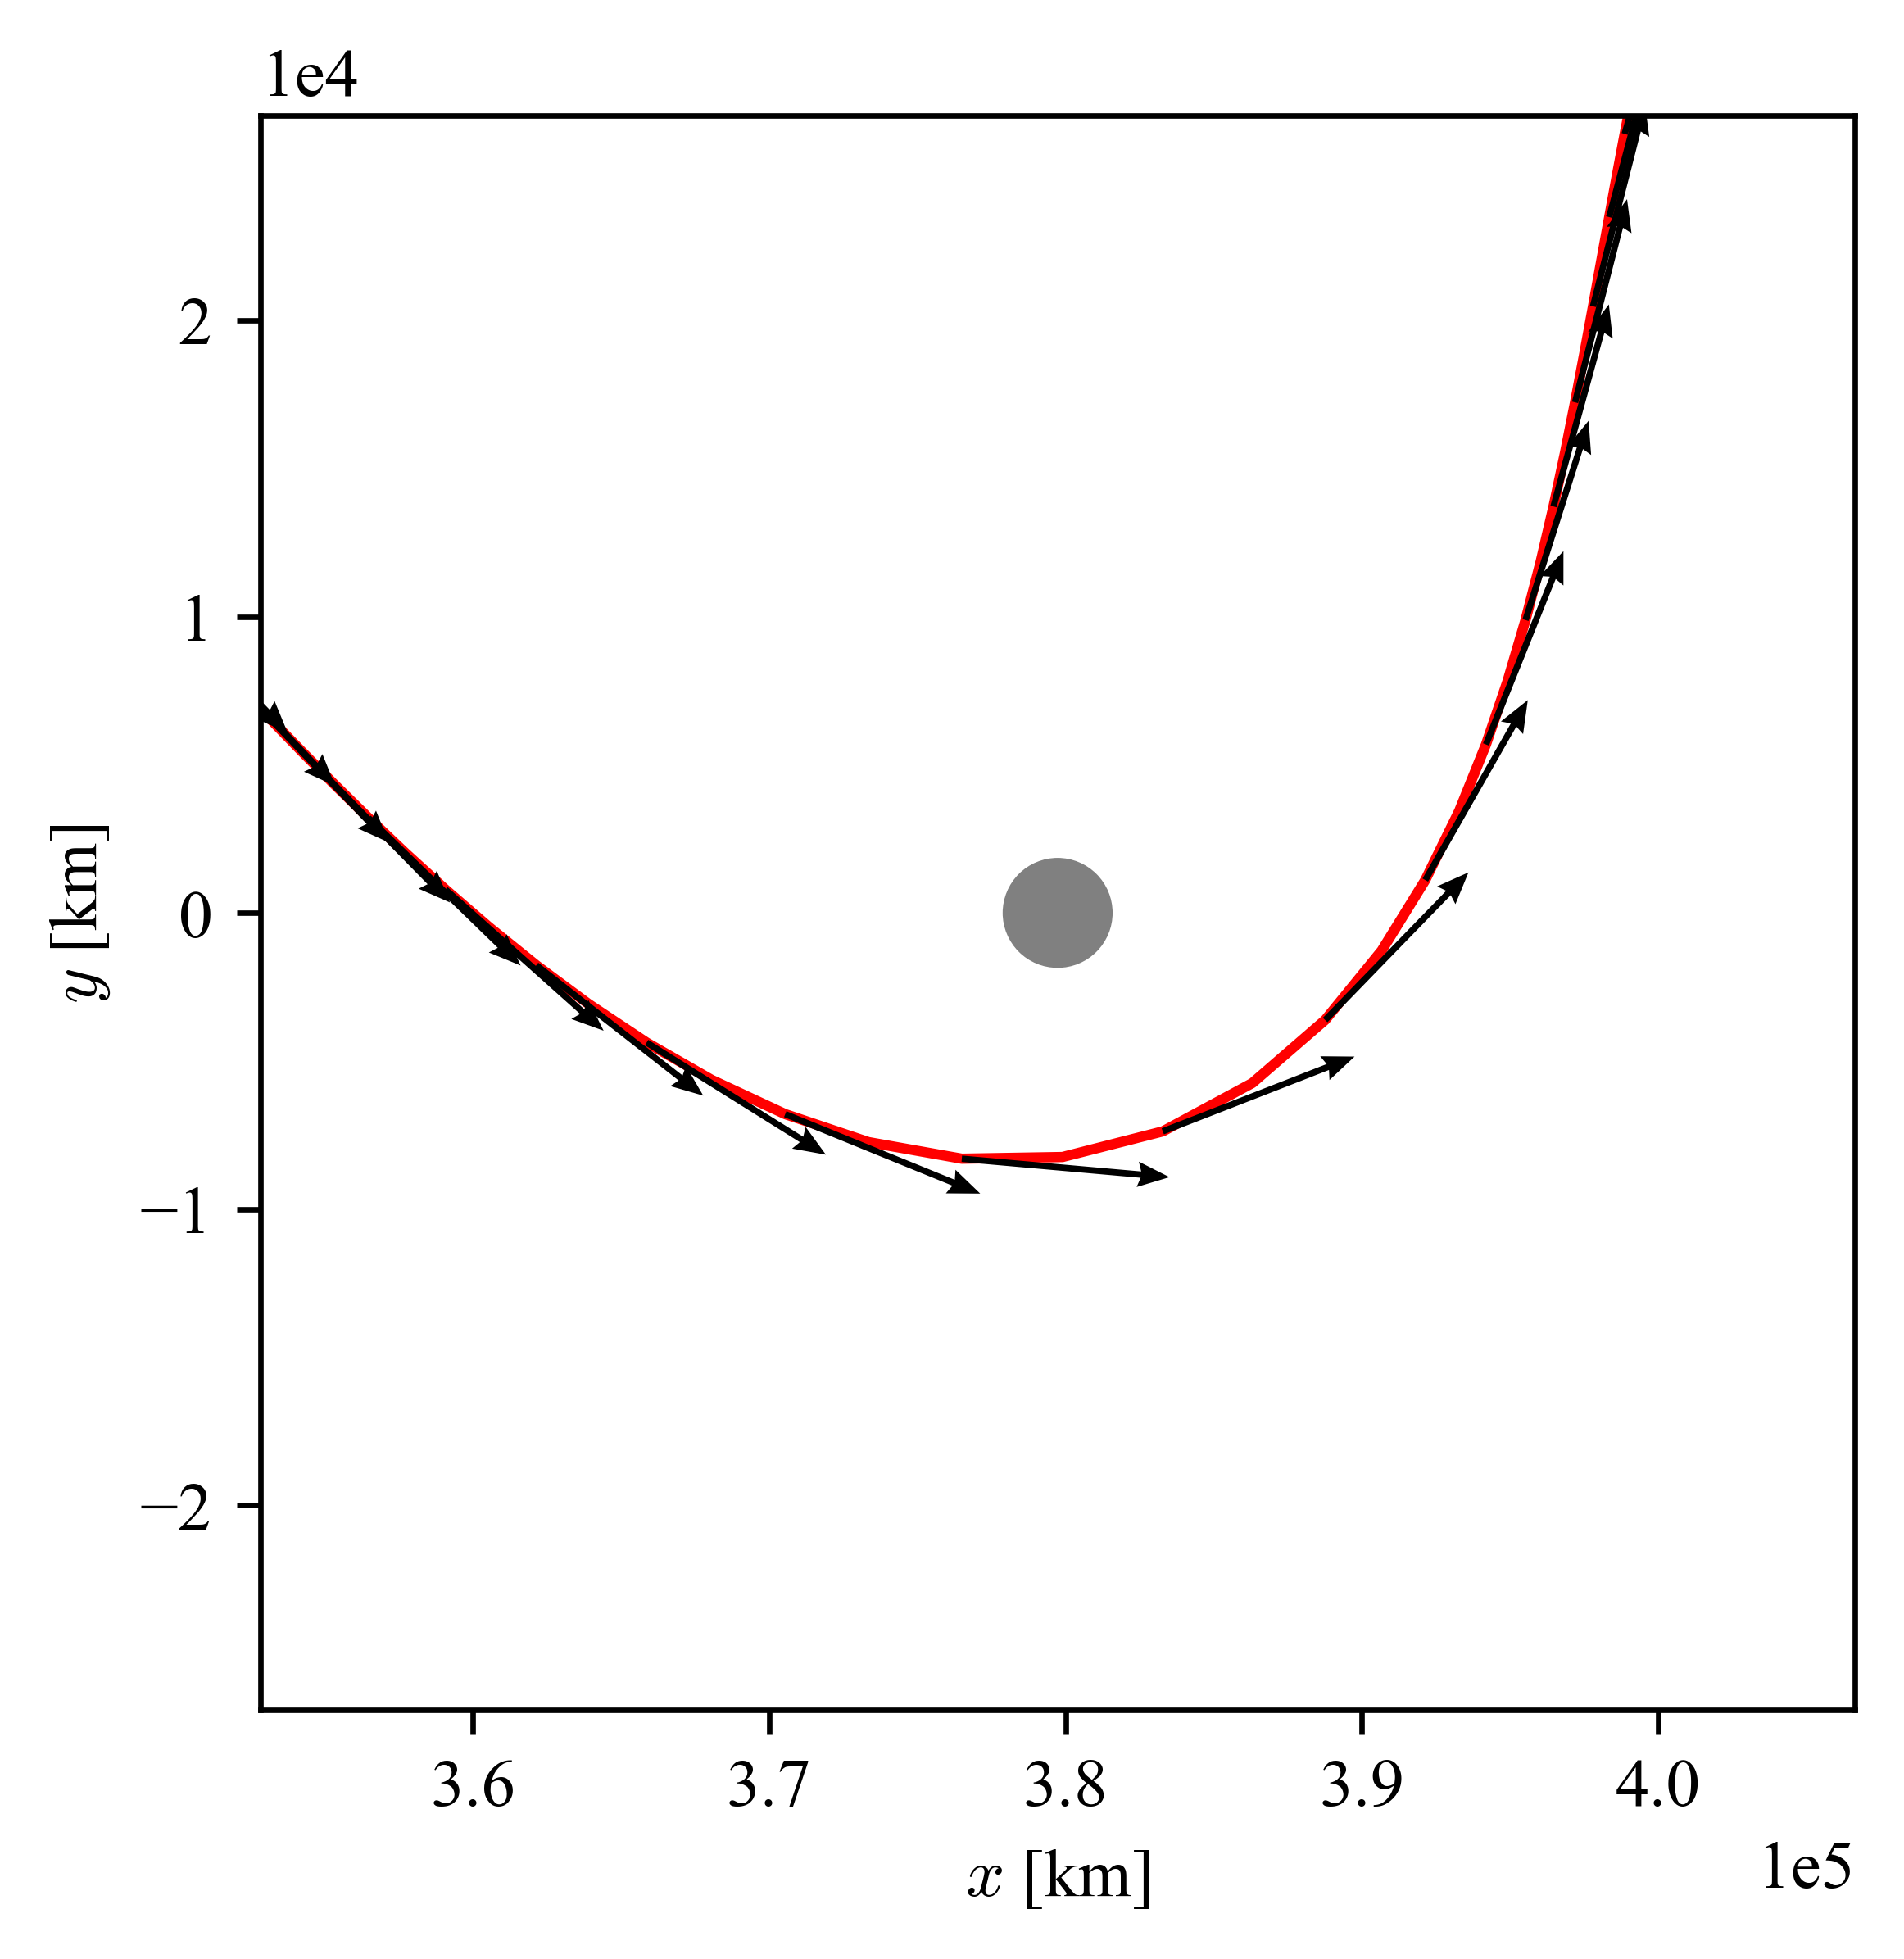
\includegraphics[width=0.4\linewidth]{Figures/closeup.png}
    \caption{Closeup of flyby maneuver, where red indicates spacecraft trajectory and black arrows indicate thrusting direction at 2 hour intervals.}
    \label{fig:closeup}
\end{figure}

To assess the estimation performance of the OCIMM, the mean absolute errors (MAEs) of  the OCIMM and acceleration IMM for the fully observed scenario are plotted in Figure \ref{fig:MAE-normal}. In general, the OCIMM and acceleration IMM have similar performance over the entire trajectory. As expected, the MAEs of both filters spike at the starts and ends of maneuvers, as the filters cannot predict when the mode will switch and must ``catch-up" to the sudden change from no control to maximum control (or vice versa) caused by the true bang-bang control profile.

The two largest differences in performance occur during the second maneuver starting at $t\approx 8$ days and during the third maneuver starting at $t\approx 13$ days. These differences in performance are caused by the difference in assumed control dynamics of the two filters. The OCIMM has worse position MAE during the third maneuver which is due to a slighly overconfident estimate, causing the OCIMM to not update its position estimate to match the measurements. This demonstrates a drawback of assuming optimal control dynamics.

On the other hand, the OCIMM has better MAE performance during the second maneuver. This is due to the high rate of change of the truth control associated with the rapidly changing geometry near the Moon, pictured in Figure \ref{fig:closeup}, as the second maneuver is a flyby maneuver. Because the OCIMM estimates the entire costate, it has some predictive power of how the control will evolve with respect to the state dynamics, so long as the true control is well-approximated by the OCIMM's assumed optimal control policy. In contrast, the acceleration IMM assumes that the control is constant (i.e. $\dot{\hat{\bm{\mu}}} = \bm{0}$), and so it has no predictive power, resulting in a lagging estimation during periods when the truth control has a high rate of change. The result is that the OCIMM outperforms the acceleration IMM during the flyby maneuver. 

\subsection{Observation Gap Scenario}

\begin{figure}
    \centering
    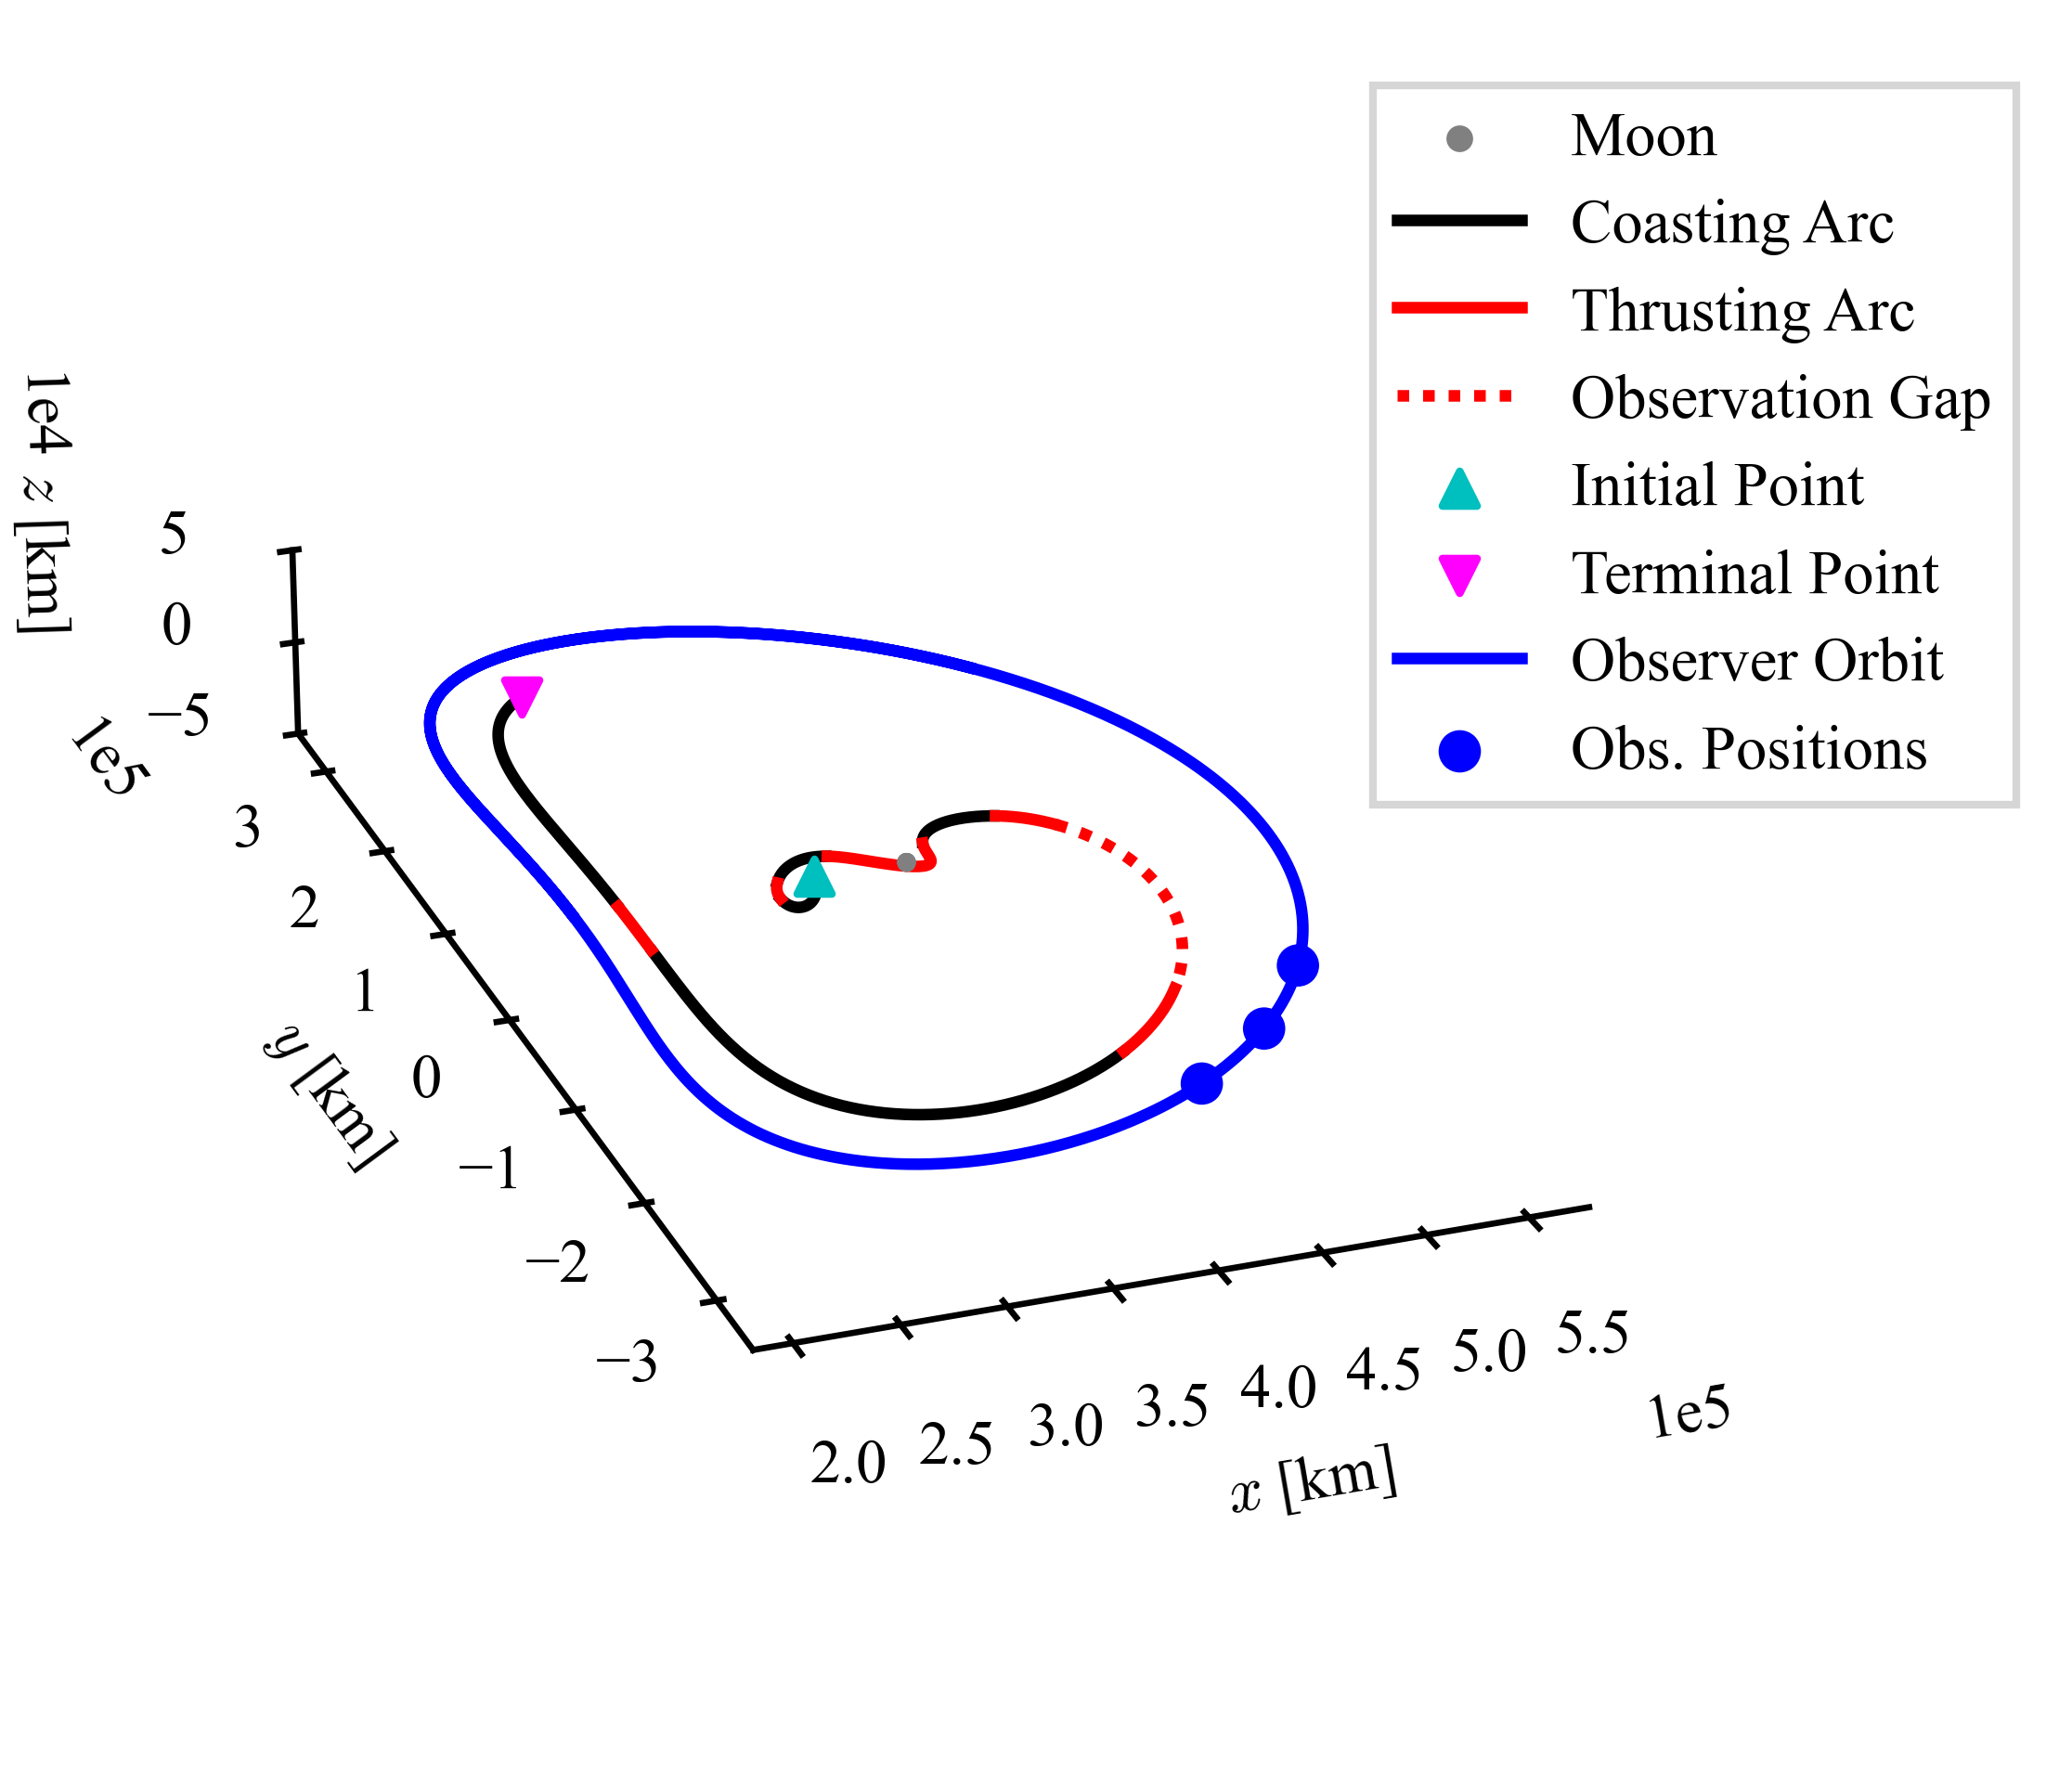
\includegraphics[width=0.5\linewidth]{Figures/unobserved_trajectory.png}
    \caption{Geometry of transfer trajectory and observers in observation gap scenario. Marked observer positions are positions of observers at beginning of the observation gap.}
    \label{fig:unobserved_trajectory}
\end{figure}

\begin{figure}
    \centering
    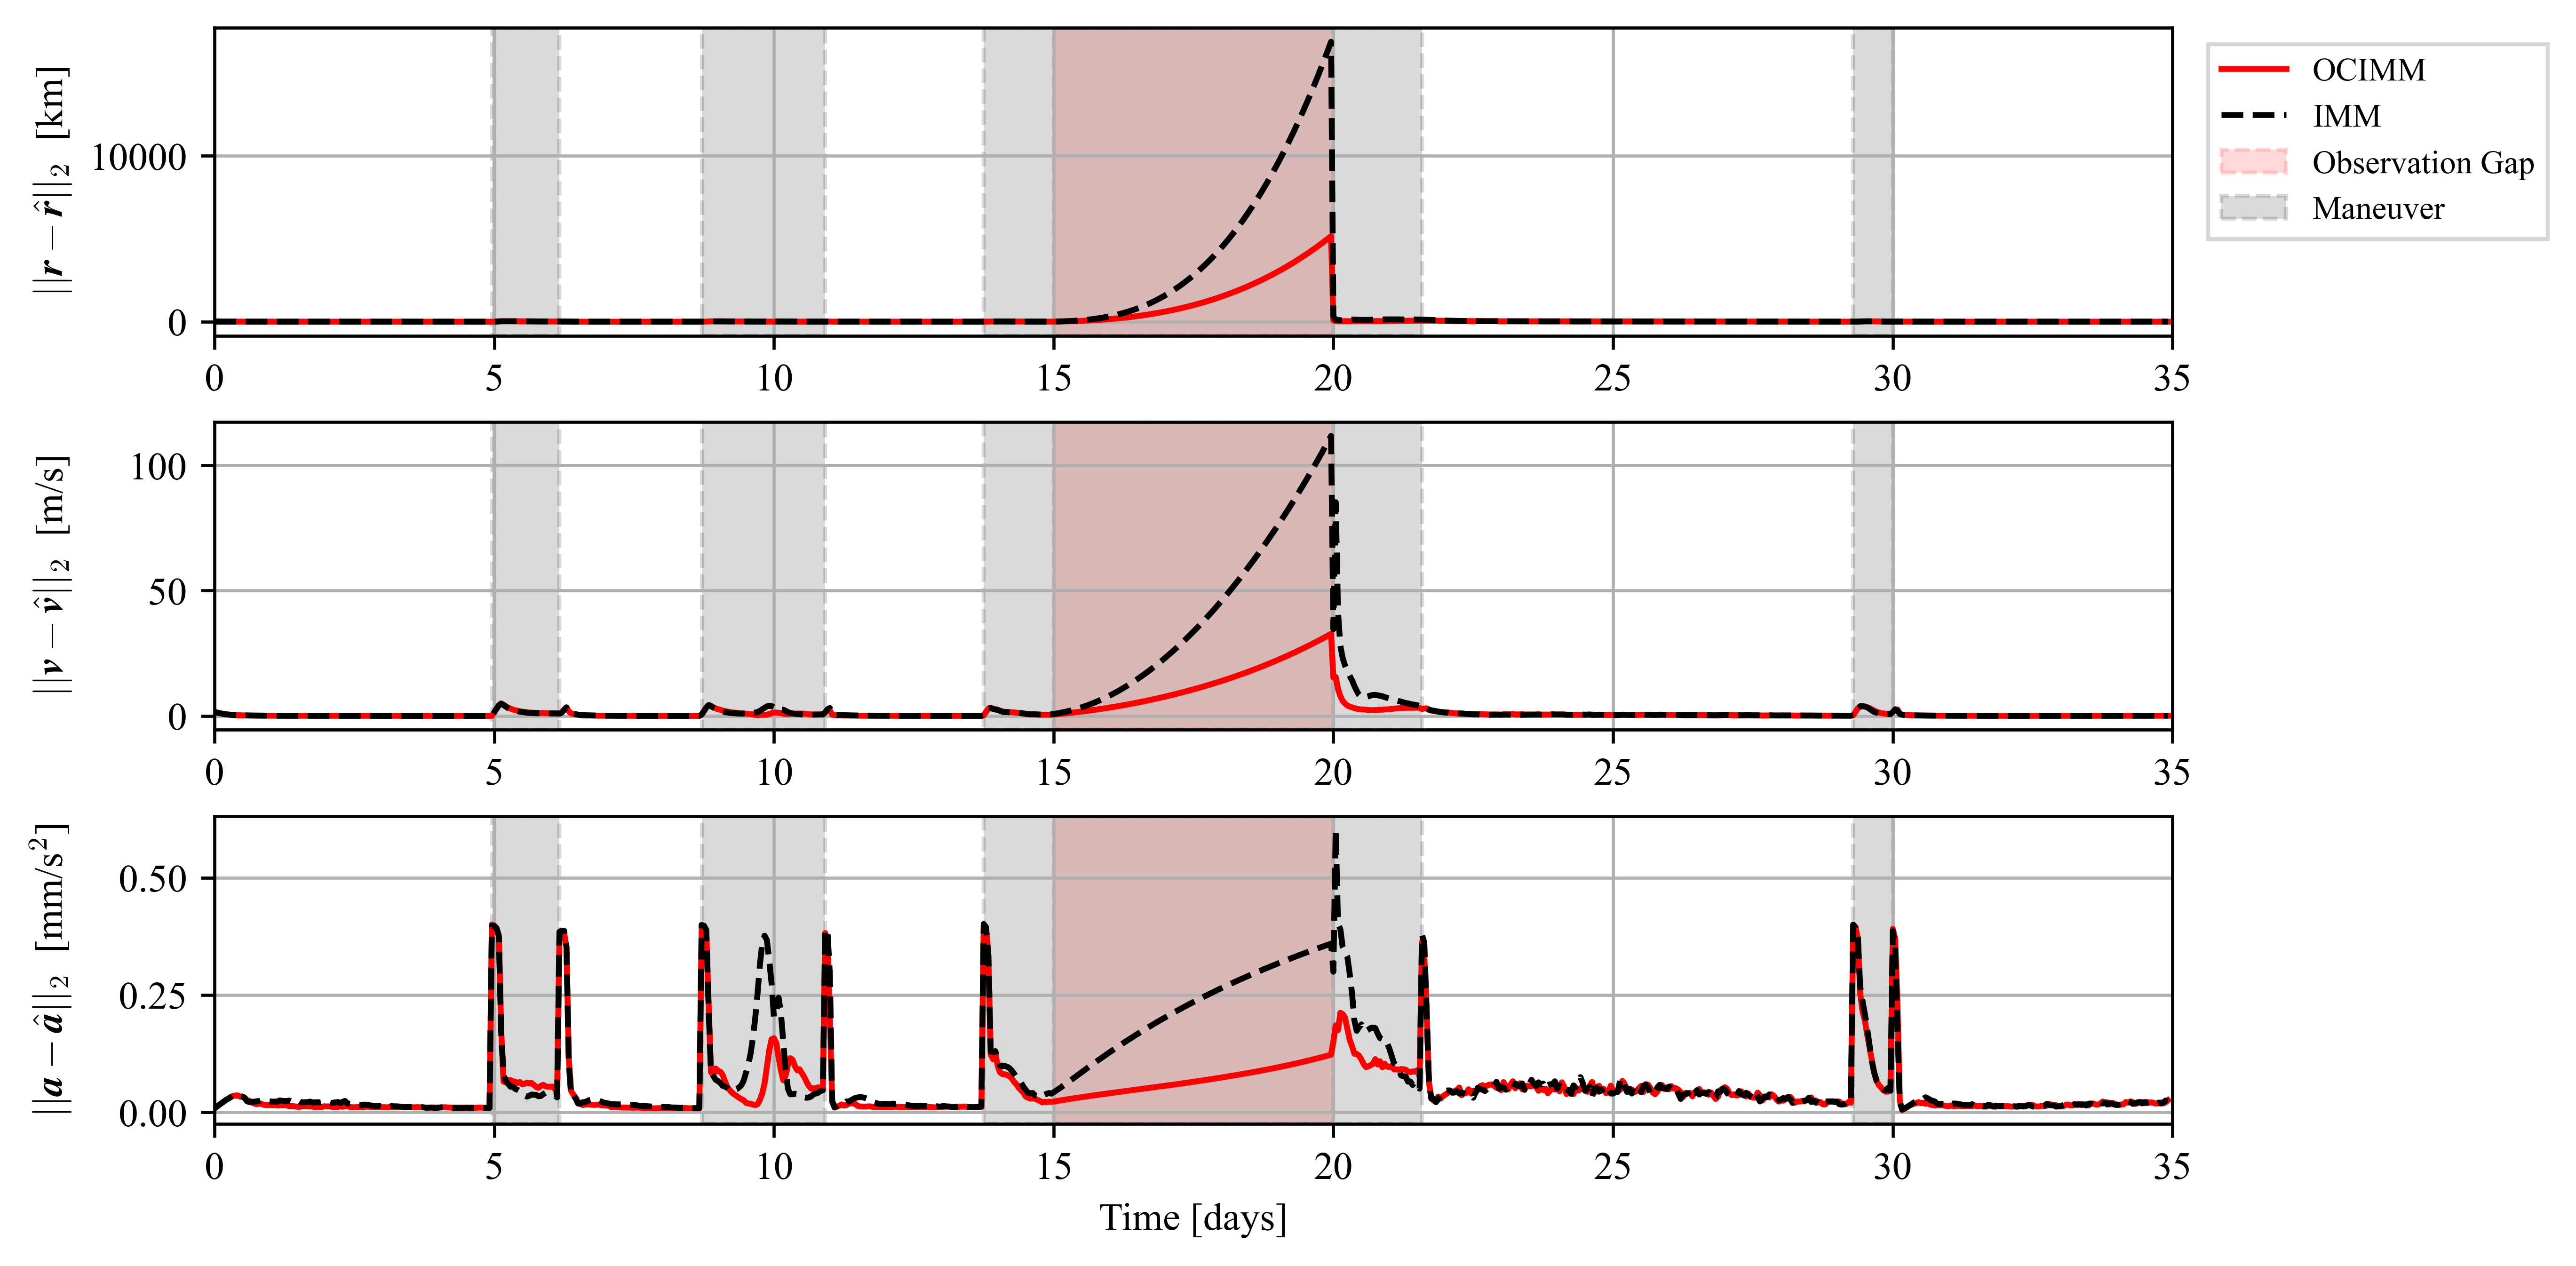
\includegraphics[width=1\linewidth]{Figures/MAE_gap.png}
    \caption{Mean absolute position, velocity, and acceleration estimation errors of acceleration IMM (black dashed lines) and OCIMM (red lines) for observation gap scenario. Grey shading indicates truth maneuvering periods and red shading indicates observation gap.}
    \label{fig:MAE-gap}
\end{figure}

\begin{figure}
    \centering
    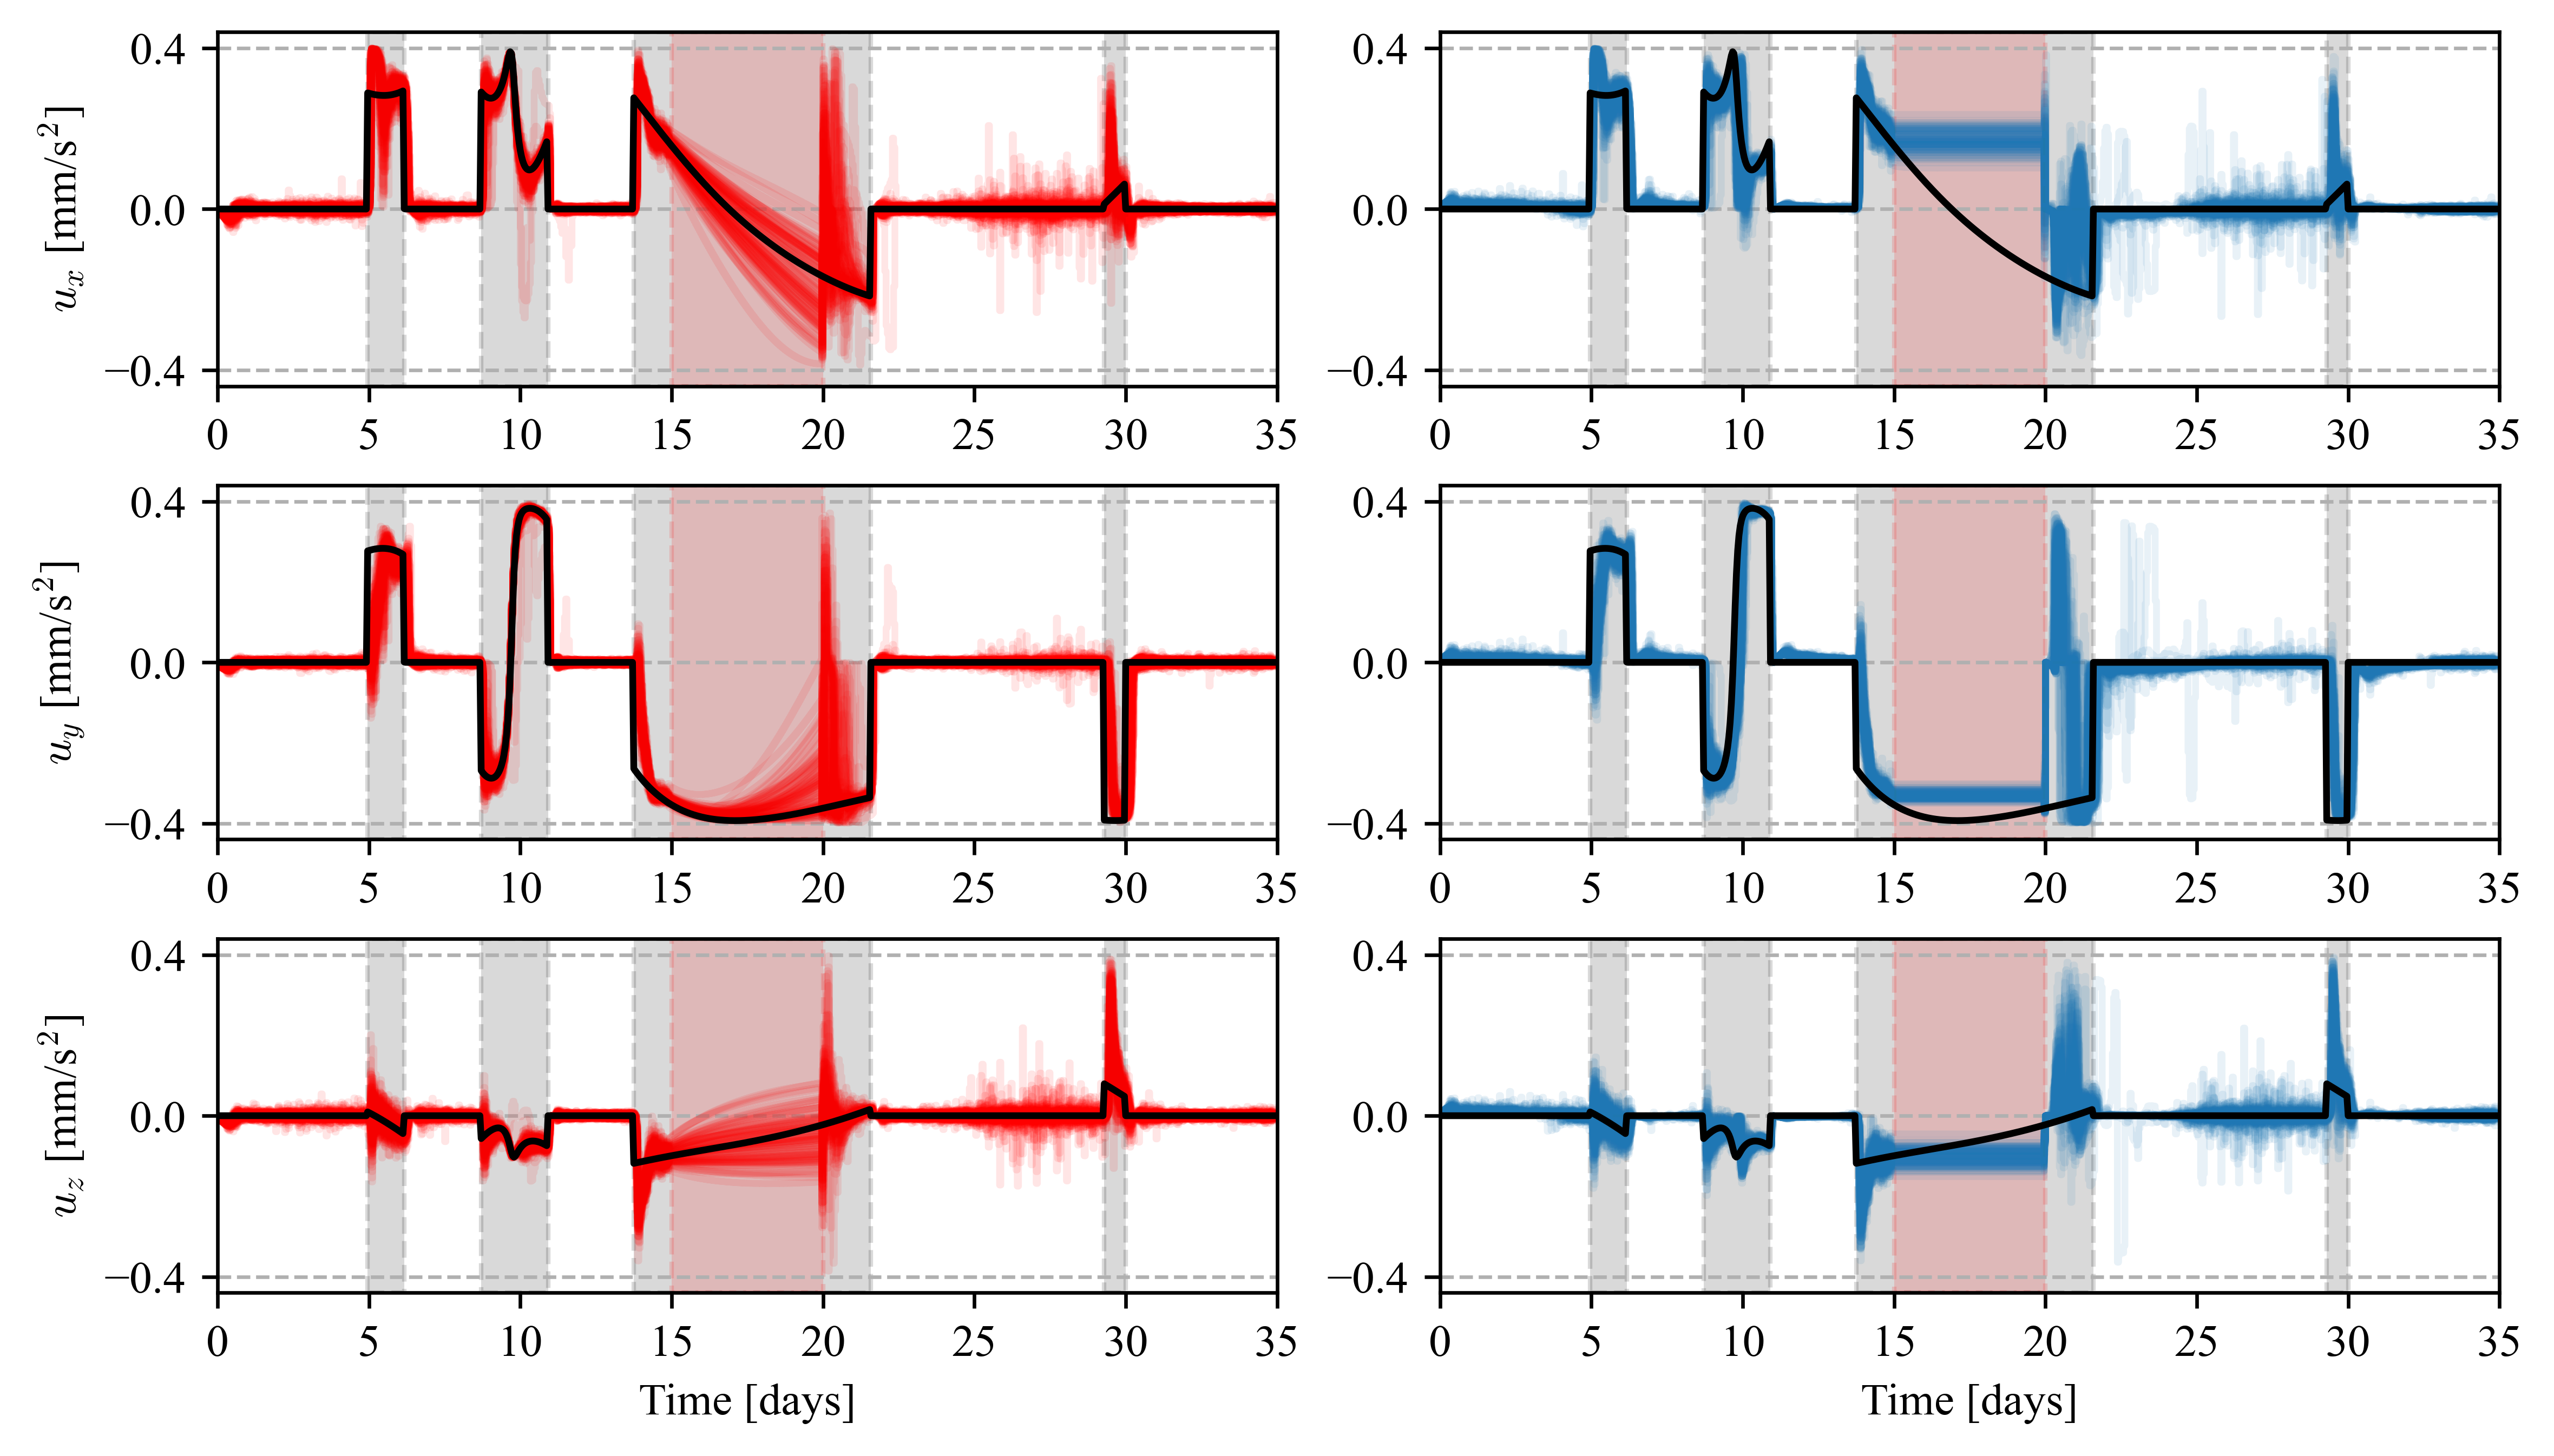
\includegraphics[width=1\linewidth]{Figures/control.png}
    \caption{Estimated control of OCIMM (red, left subplots) and acceleration IMM (blue, right subplots) over 100 Monte Carlo simulations of observation gap scenario}
    \label{fig:control}
\end{figure}

\begin{figure}
    \centering
    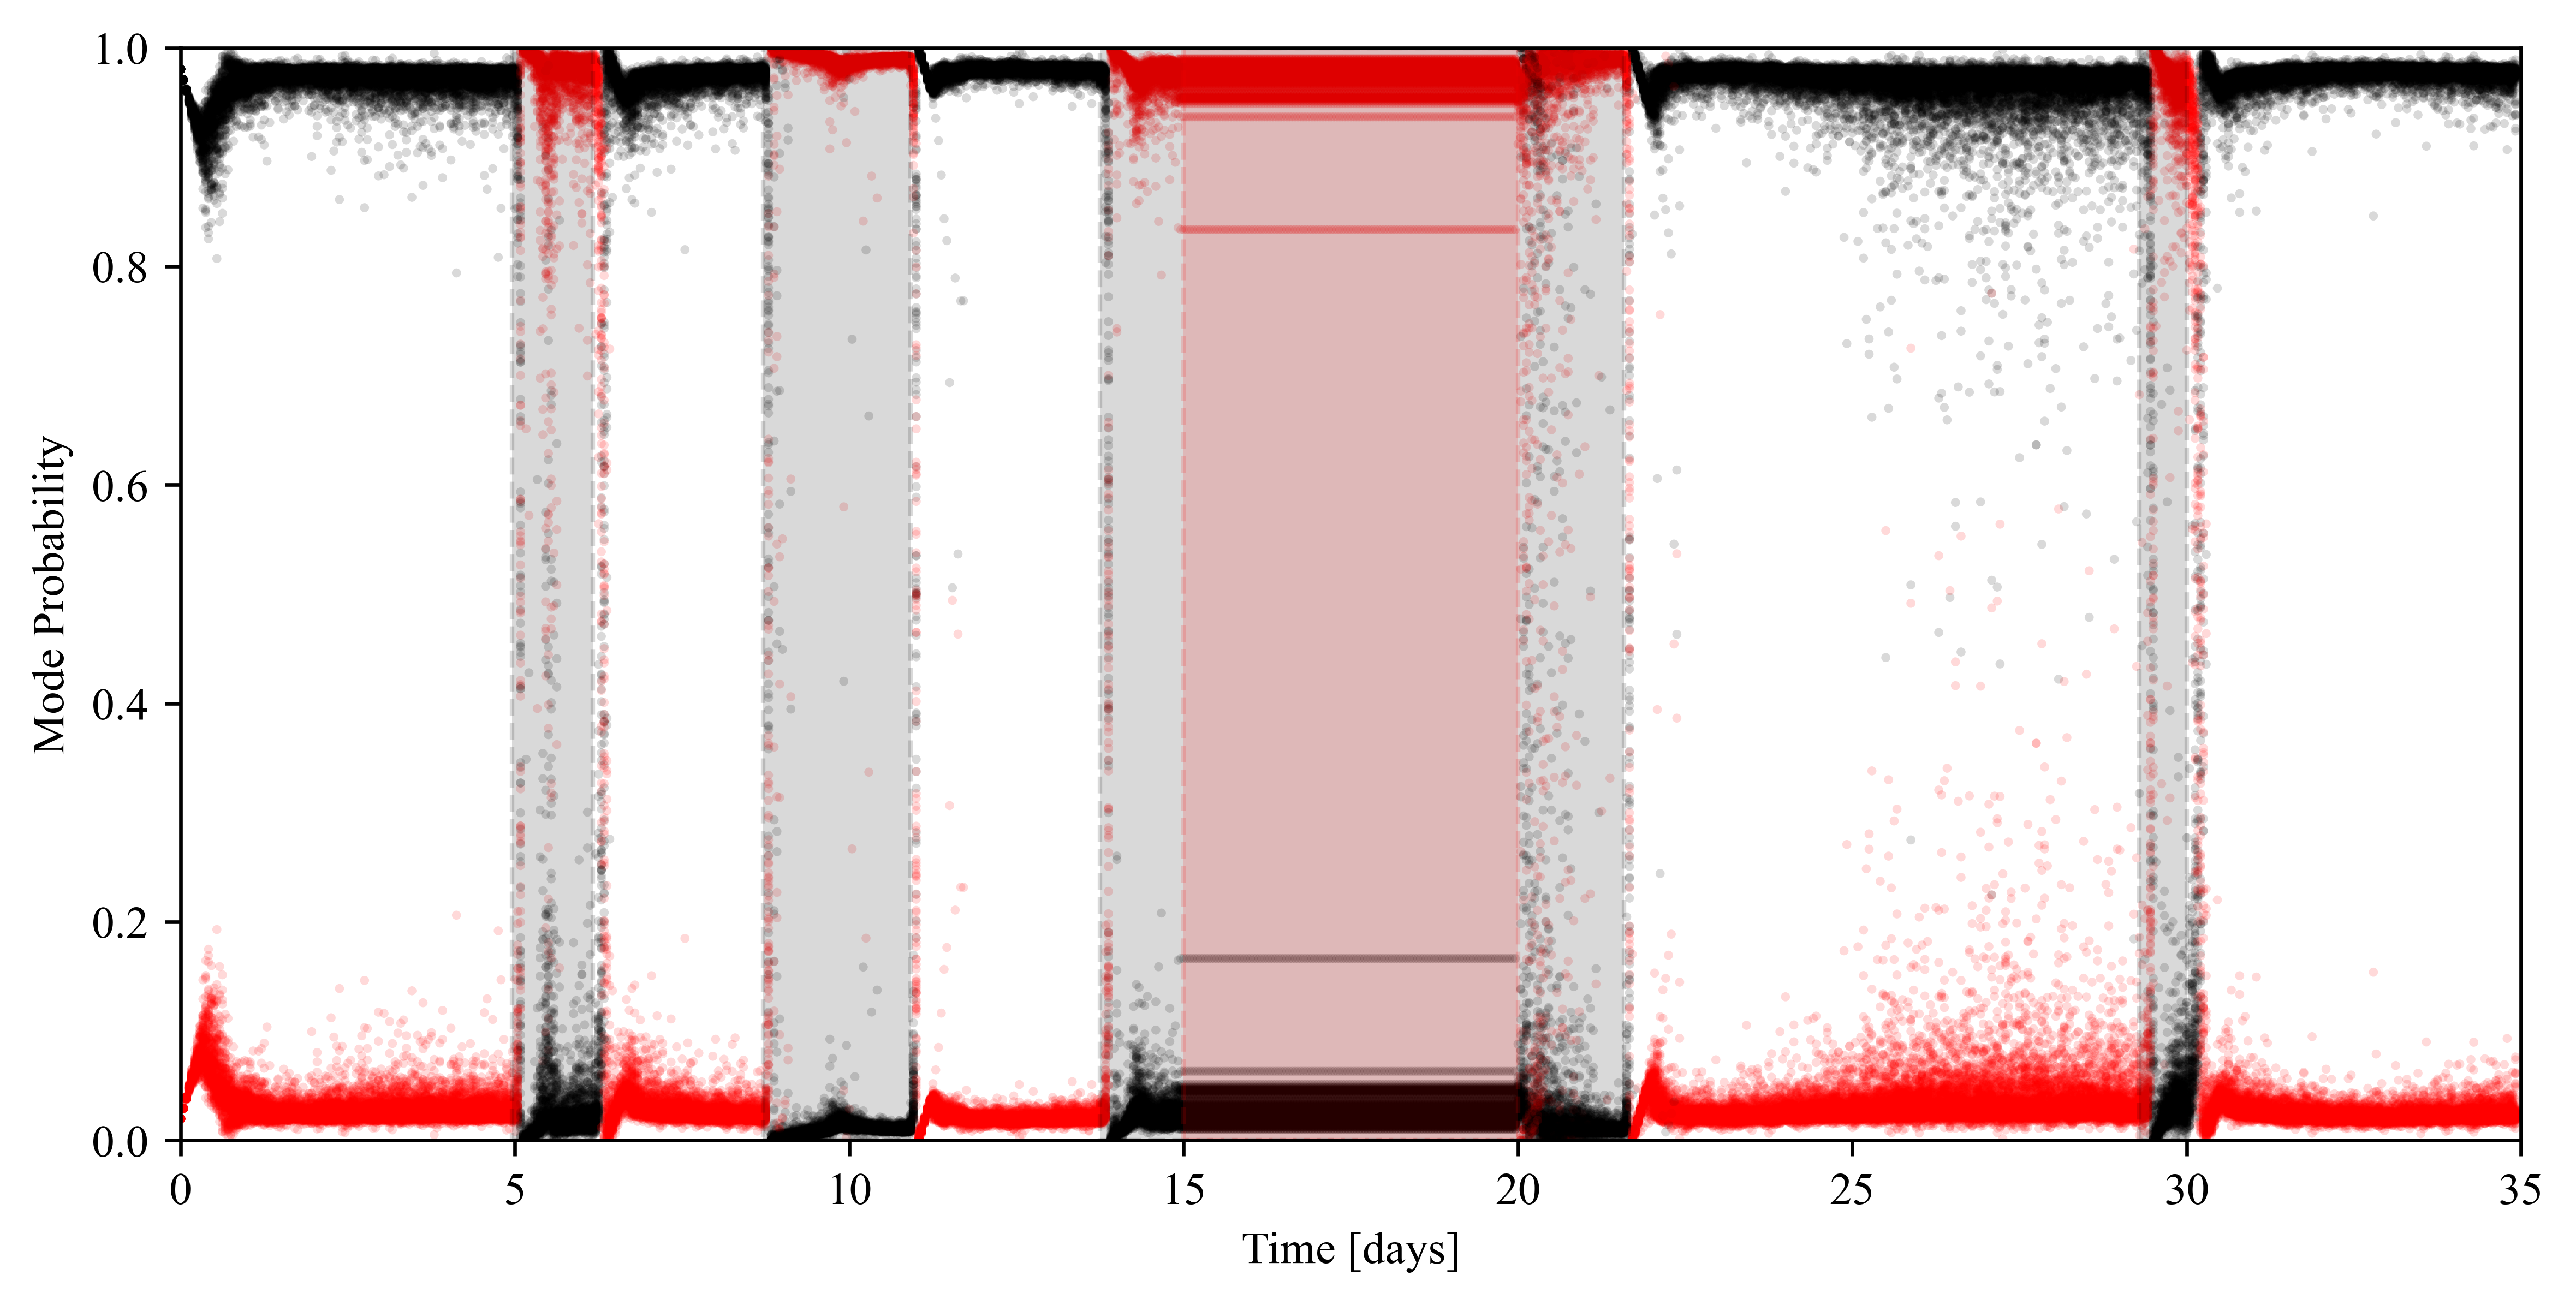
\includegraphics[width=1\linewidth]{Figures/mode_probabilities.png}
    \caption{OCIMM mode probabilities of coasting mode (black) and maneuvering mode (red) over 100 Monte Carlo simulations of observation gap scenario. Grey shading indicates truth maneuvering periods and red shading indicates observation gap. }
    \label{fig:mode-probabilities}
\end{figure}

\begin{figure}
    \centering
    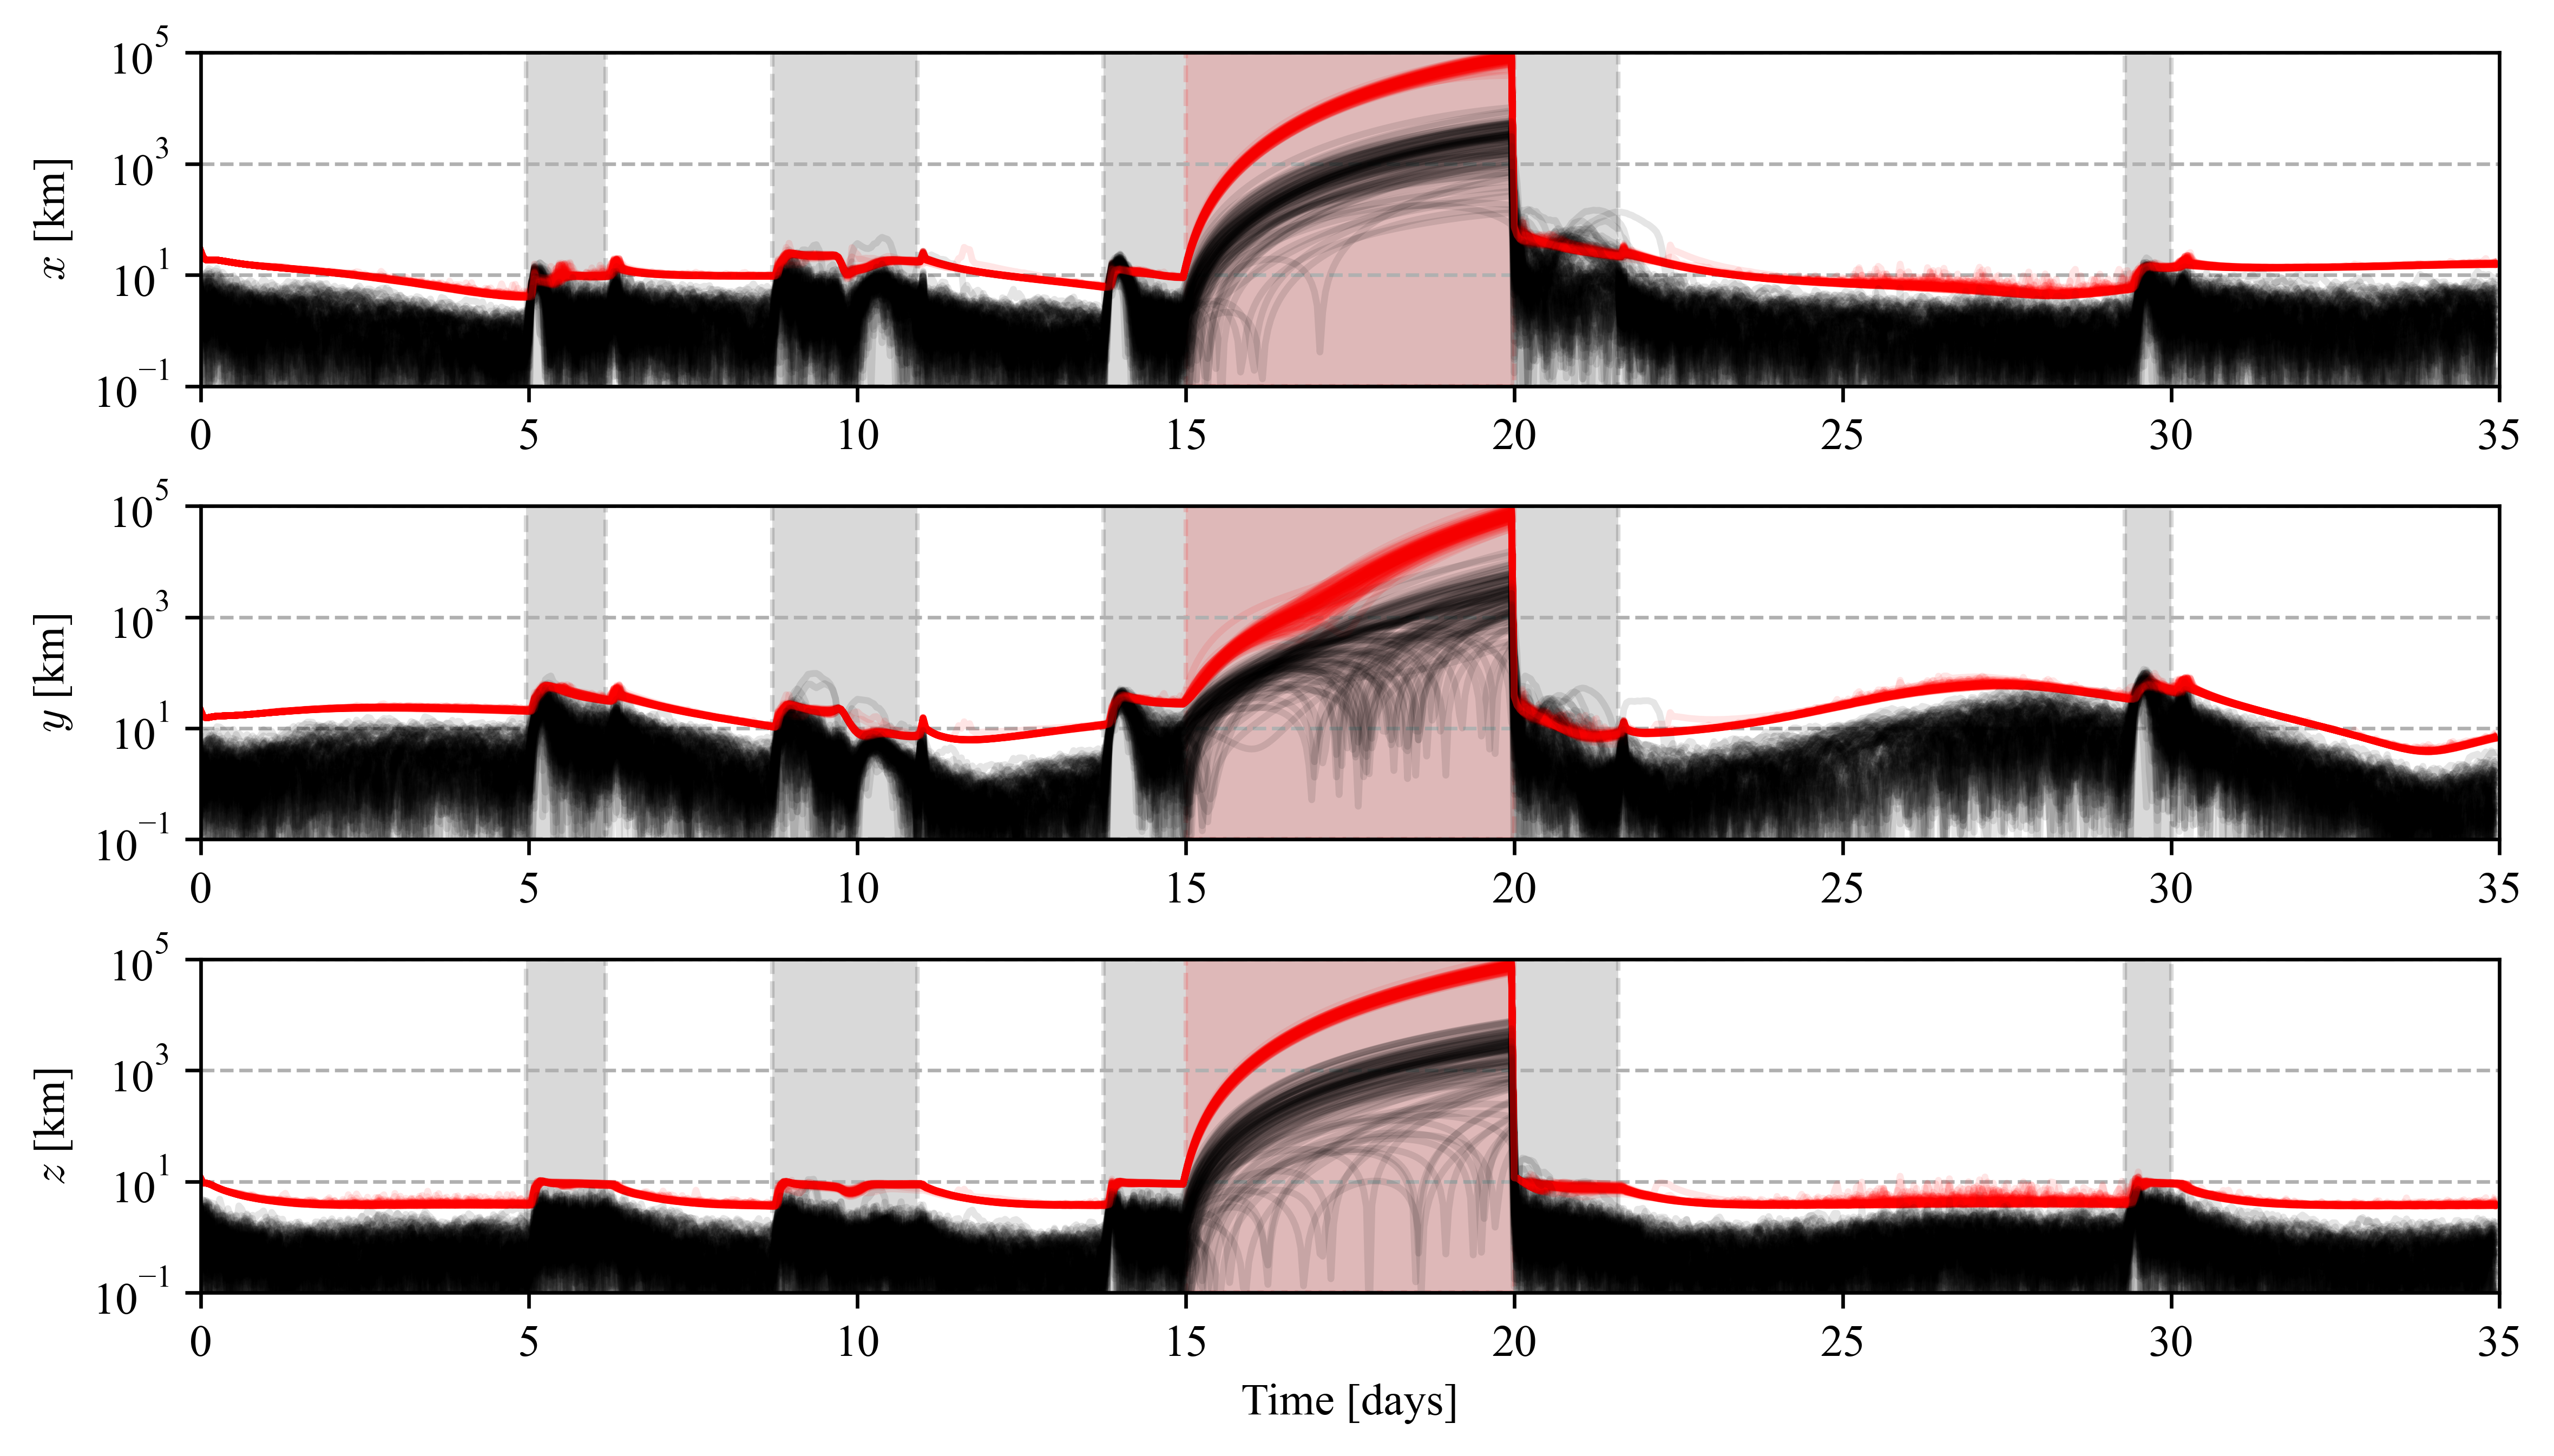
\includegraphics[width=0.85\linewidth]{Figures/position_3sigmas.png}
    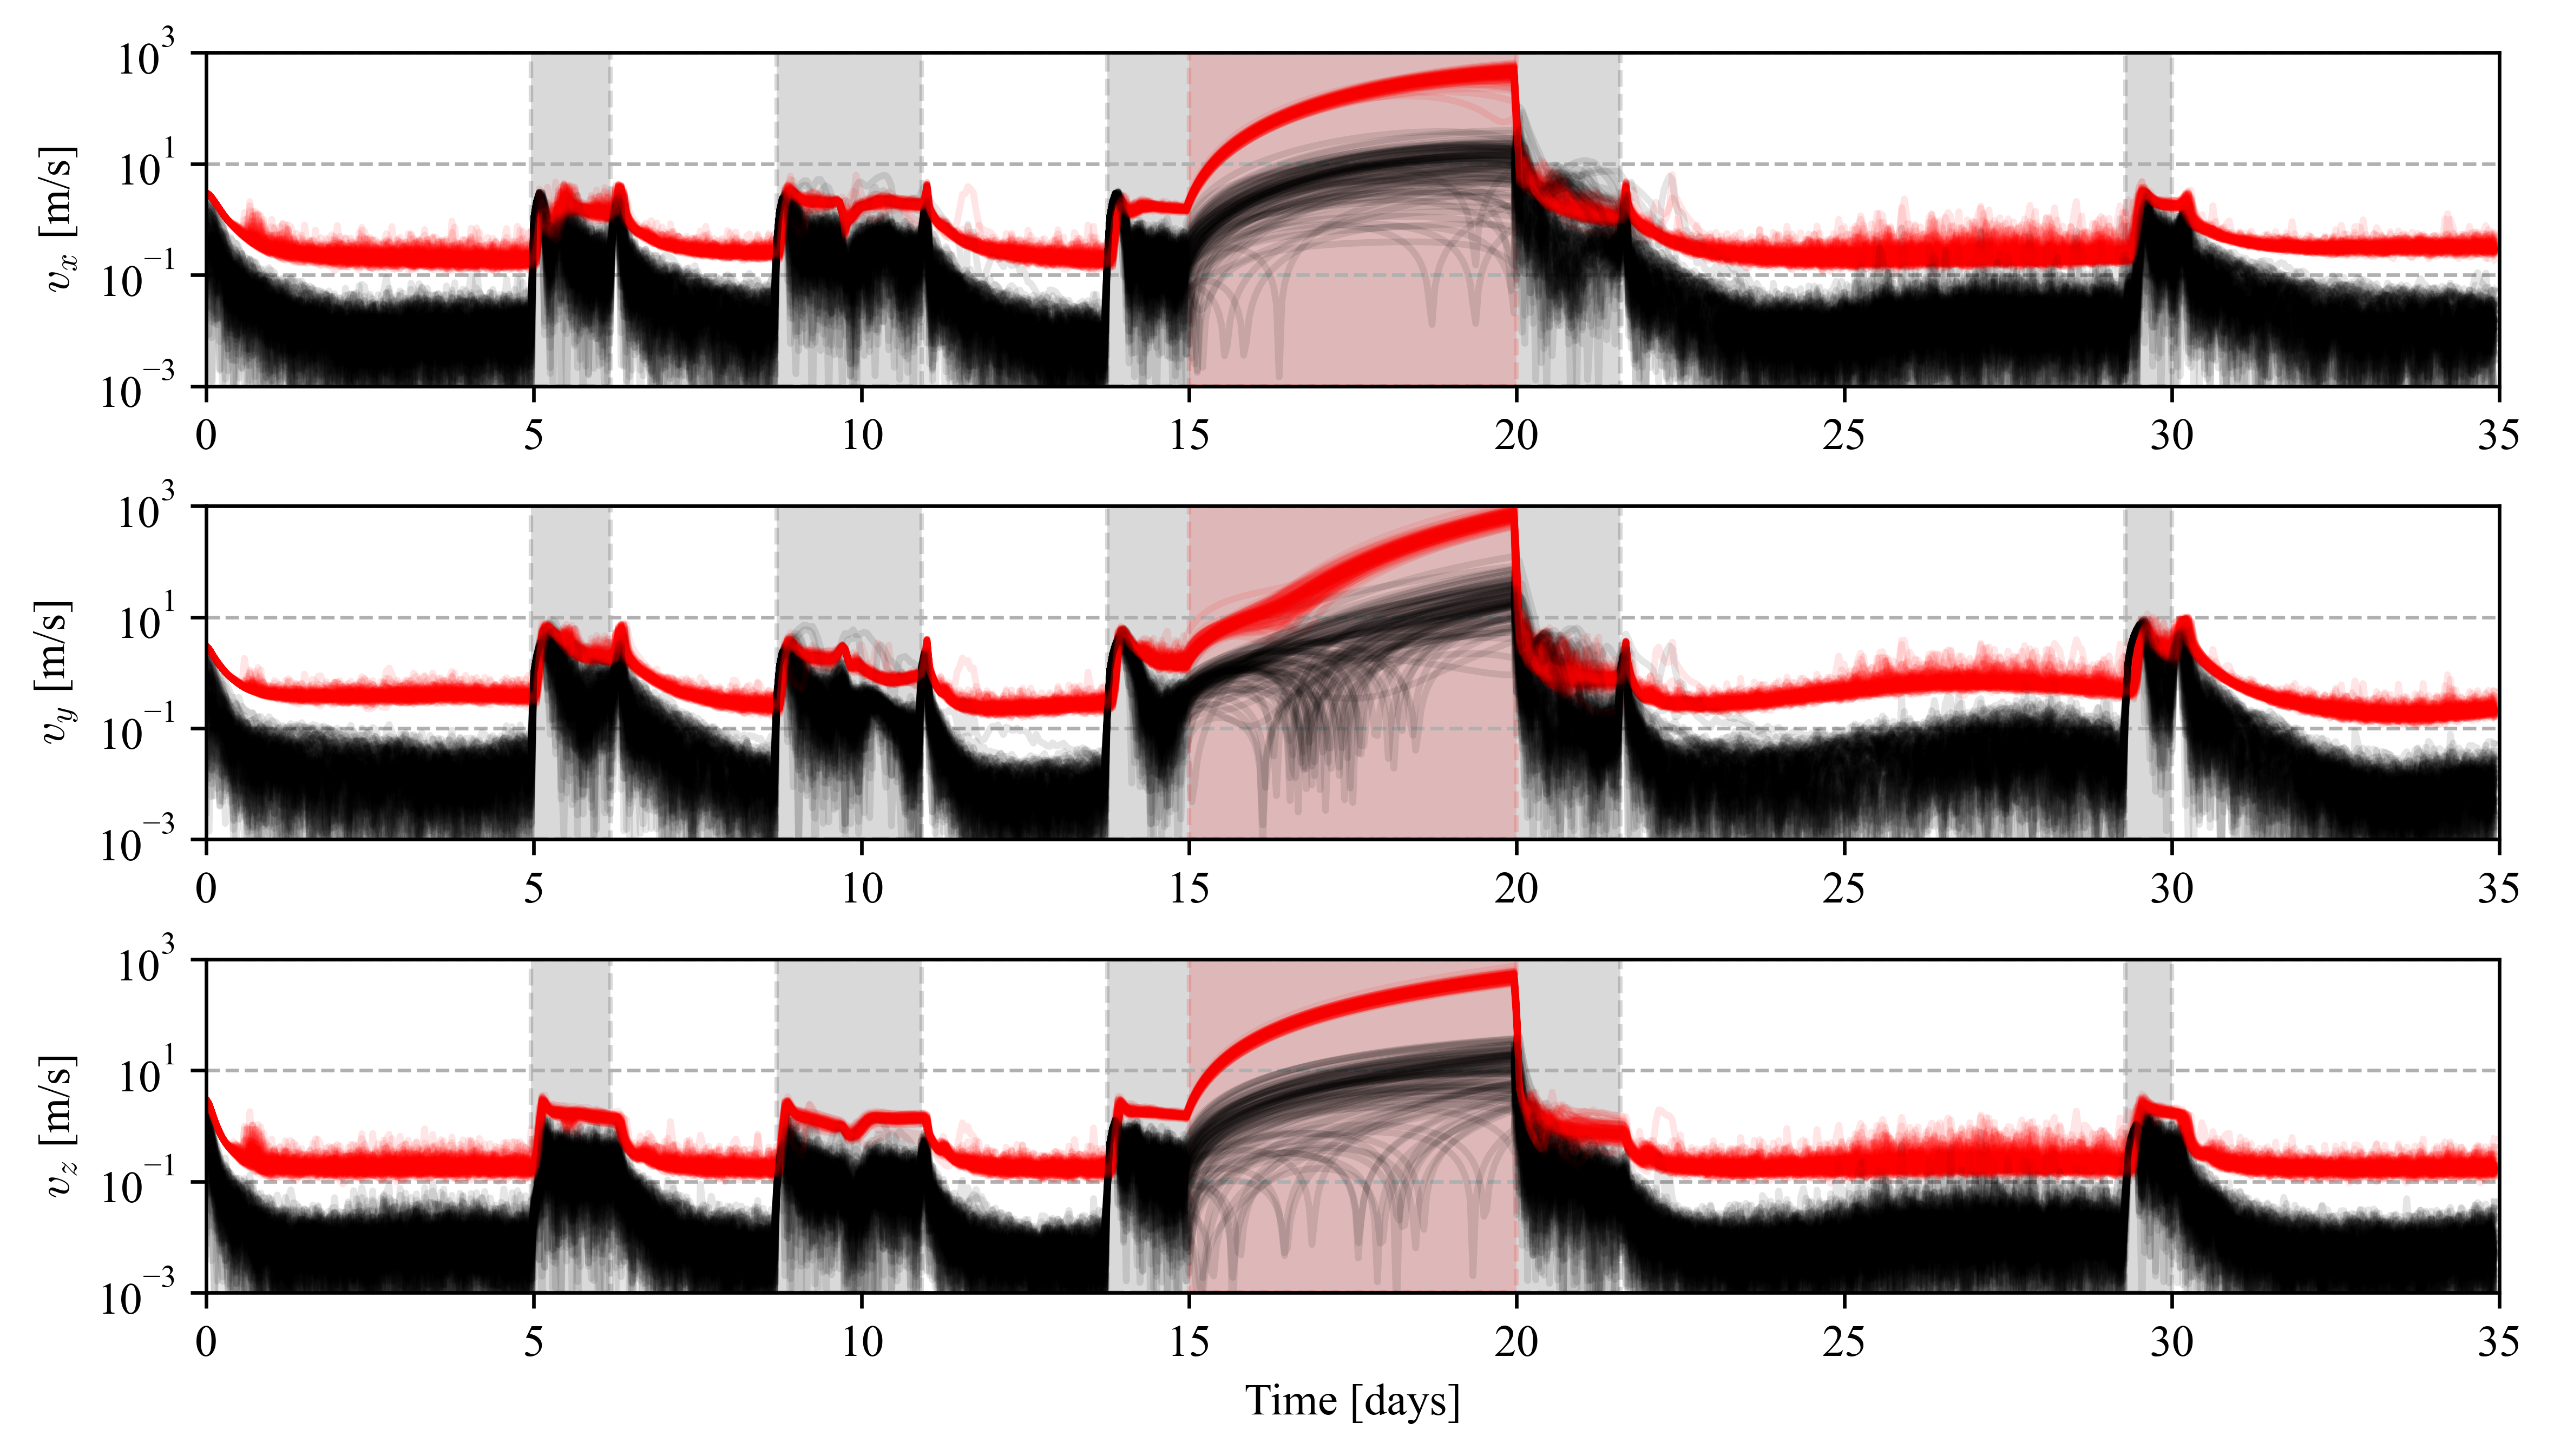
\includegraphics[width=0.85\linewidth]{Figures/velocity_3sigmas.png}
    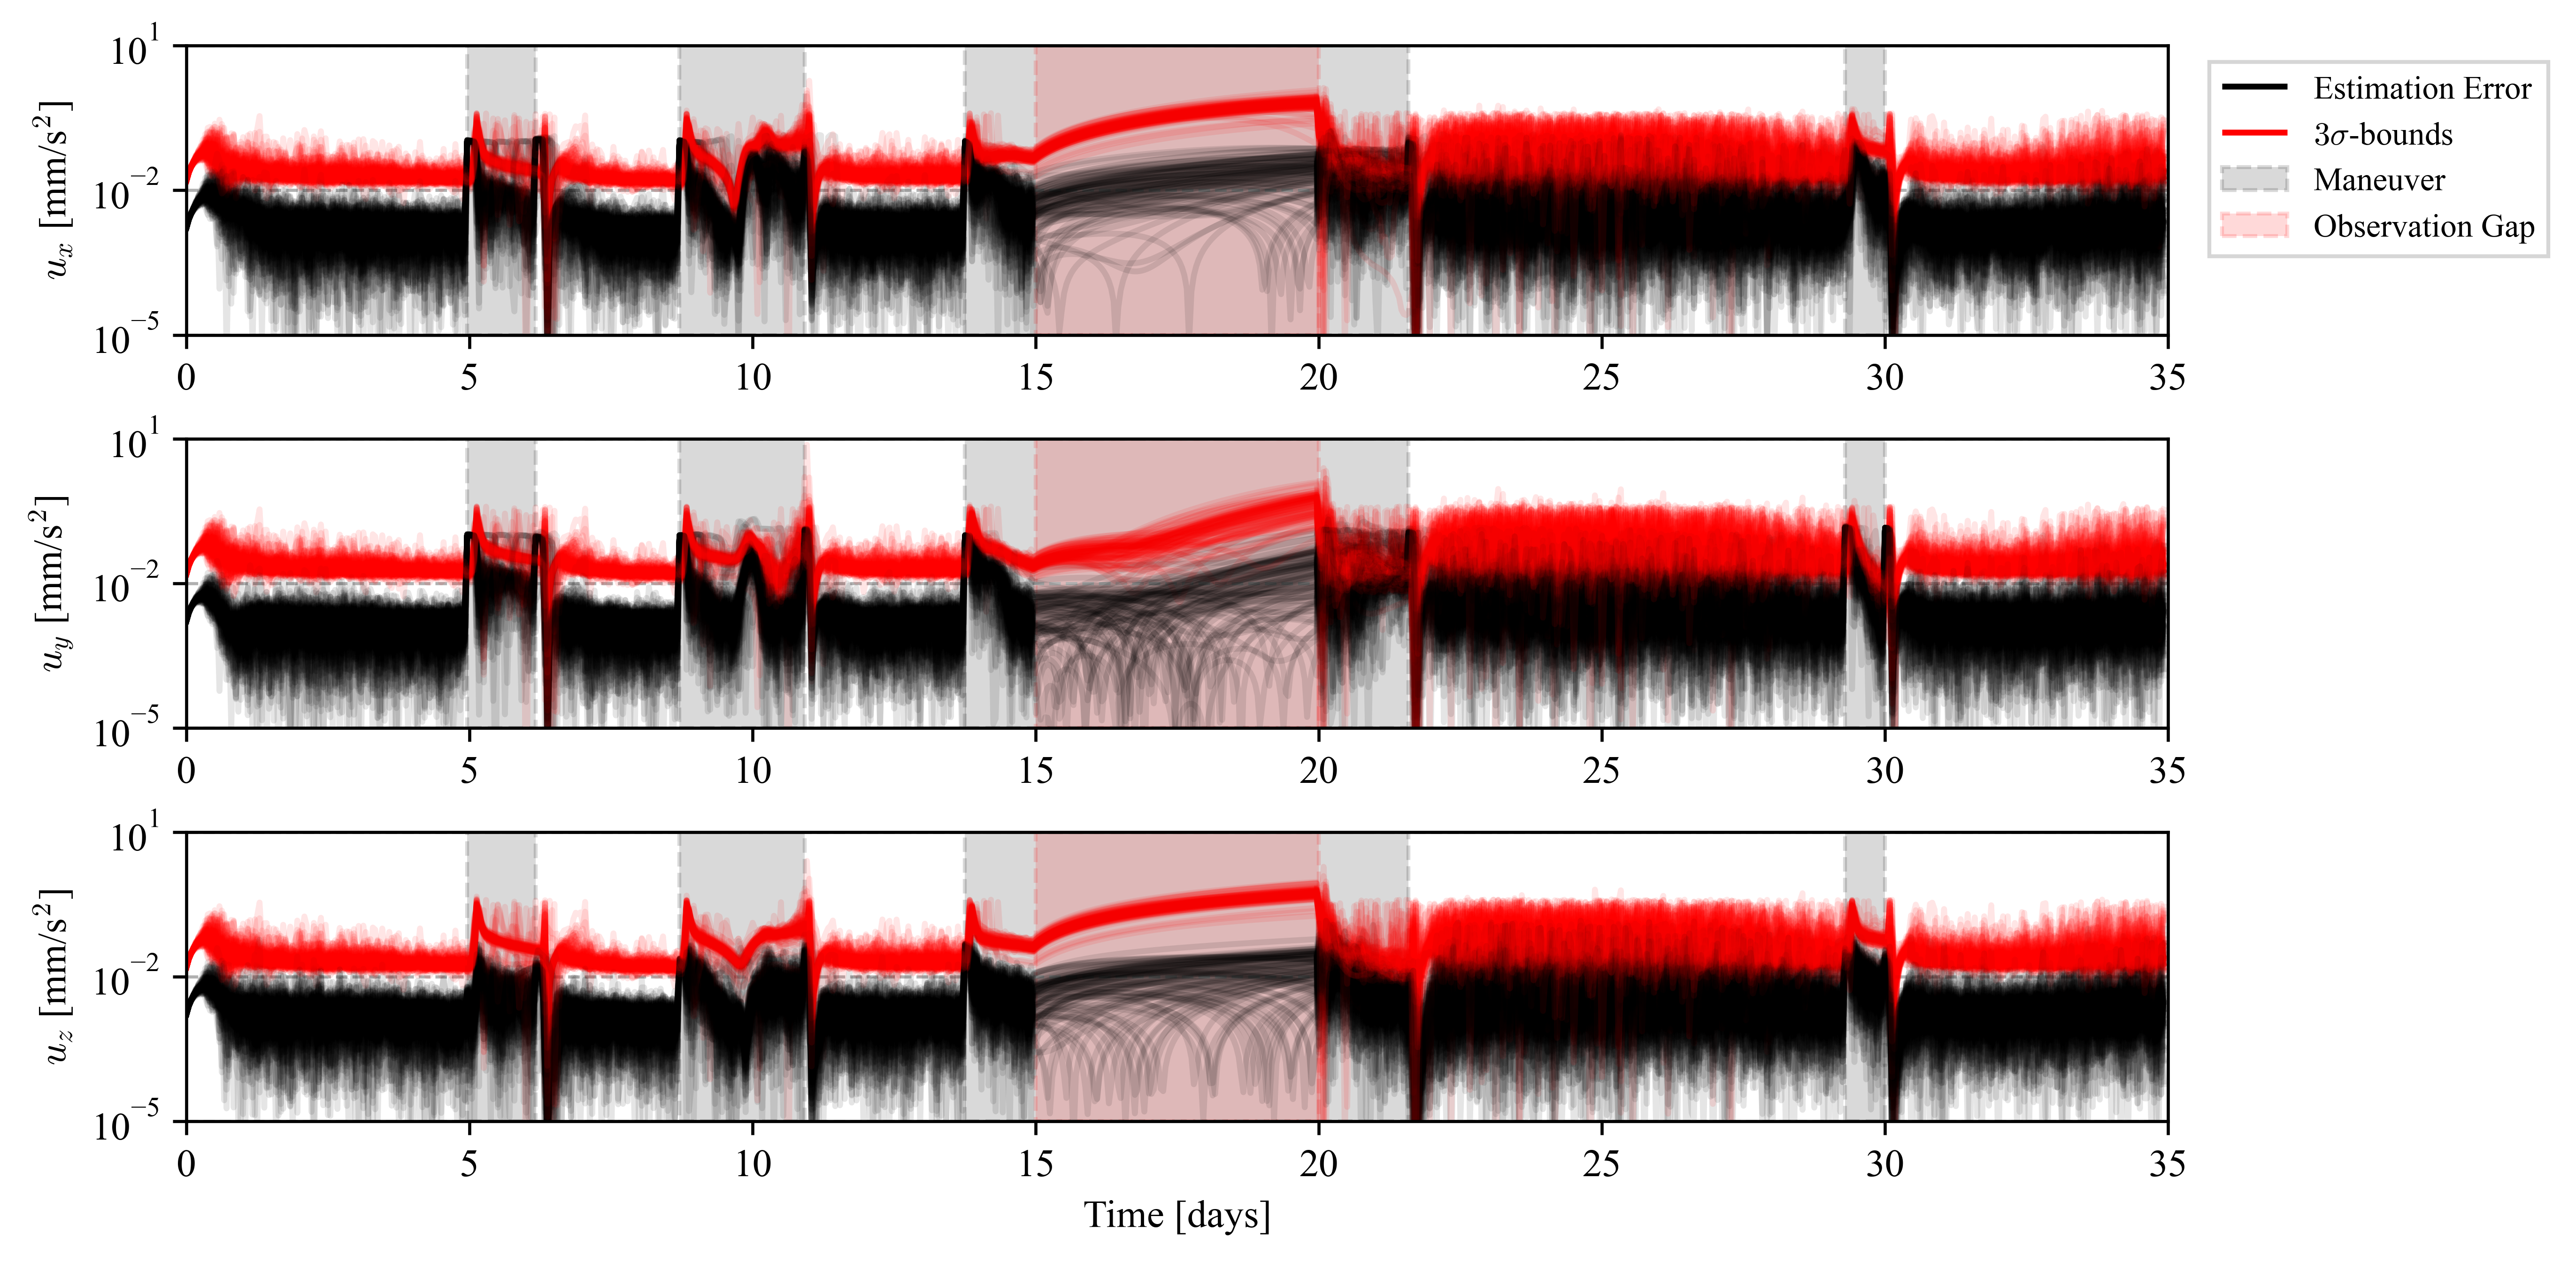
\includegraphics[width=0.85\linewidth]{Figures/control_3sigmas.png}
    \caption{Position, velocity, and control estimation errors (black lines) and estimation error $3\sigma$ bounds (red lines) of the OCIMM over 100 Monte-Carlo simulations of the observation gap scenario. Grey shading indicates truth maneuvering periods and red shading indicates observation gap.}
    \label{fig:three-sigmas}
\end{figure}

Next, to test the performance of the OCIMM during observation gaps, the MAE of position, velocity, and acceleration of the OCIMM and IMM in the observation gap scenario where observation checks are enforced are plotted in Figure \ref{fig:MAE-gap}. The geometry of the observation gap and the number of sensors over time are plotted in Figure \ref{fig:unobserved_trajectory}. While the number of sensors varies over time, we define an "observation gap" to be a period of time where no measurements are available. During the observation gap starting at $t \approx 9$ days, the OCIMM significantly outperforms the IMM. The reason for this is the ability of the OCIMM to predict the future control given some estimate of the current control. Since the observation gap occurs after the beginning of the second maneuver at $t \approx 8$ days, the OCIMM has been able to obtain some estimate of the costates given observations of the control. After the beginning of the observation gap, it is then possible to propagate the spacecraft under the assumed minimum-time optimal control dynamics. This propagation is not perfectly accurate because the control $\bm{u}$ is only a function of $\bm{\lambda}_v$, so it is difficult to obtain an accurate estimate of $\bm{\lambda}_r$. Nevertheless, the general shape of the control profile is still accurately predicted by the OCIMM.

This predictive power is demonstrated by comparing the assumed control of the OCIMM and acceleration IMM with the truth control during the observation gap, plotted in Figure \ref{fig:control}. Because of its assumed constant control, the acceleration IMM maintains its last estimated value of the control after the beginning of the observation gap at $t \approx 9$ days. In contrast, the OCIMM is able to accurately estimate the general shape of the truth control even after the beginning of the observation gap because of the inclusion of optimal control in its maneuvering mode dynamics. The result is that the OCIMM accumulates less estimation error than the acceleration IMM over the observation gap, as evidenced by their MAEs in Figure \ref{fig:MAE-gap}. 

One concern with using both the OCIMM and the acceleration IMM is that if an observation gap begins after the beginning of a maneuver, it is not known when the maneuver ends. This concern is somewhat addressed by mode mixing during the observation gap which can be observed through the mode probabilities of the OCIMM which are plotted in Figure \ref{fig:mode-probabilities}. Overall, the OCIMM's mode switching behaves as expected, with the correct mode's probability increasing suddenly after a short delay at the starts and ends of maneuvers. However, during the observation gaps without any measurement updates, the IMM's mode probability calculation causes the mode probabilites to tend toward an equilibrium determined by the mode transition matrix $\Pi$. Since the selected $\Pi$ is symmetric, the mode probabilities tend toward $\mu^{(j)} = 0.5$. This tendency towards equilibrium can be thought of as greater uncertainty in the mode as the observation gap continues, and the discrete mixing allows both the possibility of coasting and thrusting to be considered in the state estimate. At the end of the observation gap, there is some noisy behavior as the estimators recover from the large innovations caused by the lack of measurements. The noisy behavior starting at $t \approx 25$ days is due to the geometry of the observers during that period, as their alignment relative to the target yields poor range information. This is also exhibited by a corresponding increase in position MAE as seen in Figure \ref{fig:MAE-normal}.


Lastly, to assess the consistency of the OCIMM, its estimation error and estimation error $3\sigma$ bounds from the observation gap scenario are plotted in Figure \ref{fig:three-sigmas}. Since the OCIMM is estimating the costate, the covariance of the control must be obtained by linearly transforming the costate covariance. This transformation is described in Eq. \ref{eq:covariance-transform},
\begin{align}
    P_{u, k} = U_kP_{\bm{\lambda}_v, k}U_k^\top, \quad U_k = \left. \frac{\partial \bm{u}(\bm{\lambda})}{\partial{\bm{\lambda}}} \right|_{\bm{\lambda}=\hat{\bm{\lambda}}_k}, \quad \bm{u}(\bm{\lambda}) = -u_\text{max} \frac{B^\top \bm{\lambda}}{\norm{B^\top \bm{\lambda}}_2} \label{eq:covariance-transform}
\end{align}
\noindent where $P_{u,k} \approx \E[(\bm{u} - \hat{\bm{u}})(\bm{u} - \hat{\bm{u}})^\top] \in \R^{3 \times 3}$ is the control covariance matrix, and $P_{\bm{\lambda}_v} \in \R^{3 \times 3}$ is the portion of ${}^+P_k$ corresponding to the estimate of $\bm{\lambda}_v$. 

It can be seen that the OCIMM is able to mostly maintain convergence when directly estimating the costate, even in periods of rapidly changing control and after observation gaps. This demonstrates the validity of an estimation approach which directly implements the costate in the state vector. There are periods when the estimation error exceeds the three sigma bounds, particularly during the first maneuver and the third maneuver. The first maneuver can be

\section{Conclusion}

This paper presents the tracking of a low-thrust, maneuvering spacecraft in cislunar space with the implementation of an assumed optimal control policy directly into a sequential filter through the combination of Pontryagin's Minimum Principle and the interacting multiple model estimator (IMM). The resulting optimal control IMM (OCIMM) is able to accurately predict the control input of a low-thrust maneuvering spacecraft in cislunar space maneuvering under an bang-bang, fuel-minimum control policy, even in the presence of rapidly changing control inputs and observation gaps. This predictive power results in superior performance compared to a traditional acceleration IMM. 

There are several opportunities to improve the presented work. Additional models can be implemented into the IMM to simultaneously account for more possible control policies, as the current implementation assumes only a single optimal control policy. Principles of the variable state dimension filter can be implemented to account for the estimation error spikes at the starts and ends of coasting arcs while also allowing for a more accurate initial guess of the costate at the beginning of maneuvers. Finally, the presented work assumes that the maximum acceleration of the spacecraft $u_\text{max}$ is known, so an improved estimator could be designed to simultaneously estimate this maximum thrust along with the spacecraft states and costates. 

\bibliographystyle{AAS_publication}   % Number the references.
\bibliography{references}   % Use references.bib to resolve the labels.



\end{document}
